\documentclass[oneside,twocolumn]{book}

\usepackage{Qstyle}		% to include mystyle.sty, where I put all my \newcommand statements, etc.

%\includeonly{}			% if I want to process just {}.tex
%\syntaxonly										% if I want to process just the syntax
%\doublespacing									% if I want to double space the entire document
\makeindex											% to make an index
%\makeglossaries									% to make a glossary

\begin{document}

\begin{titlepage}

\begin{center}


% Upper part of the page

\includegraphics[width=0.15\textwidth]{TTULogo2.jpg}\\[1cm]

\textsc{\LARGE Tennessee Technological \\[2mm] University}\\[1.5cm]

\textsc{\Large Dr.\ Connie Hood's Mentor Group \\ Level 1}\\[0.5cm]

% Title
\HRule \\[0.4cm]
{ \huge \bfseries Mentor Handbook 2007-2008}\\[4mm]
{ \Large a guide to the point of departure}\\[2mm]

\HRule \\[1.5cm]

% Author and supervisor
\begin{minipage}{0.4\textwidth}
\begin{flushleft} \large
\emph{Typesetter:}\\
Quinton \textsc{Westrich}
\end{flushleft}
\end{minipage}
\begin{minipage}{0.4\textwidth}
\begin{flushright} \large
\emph{Supervisor:} \\
Dr. Connie \textsc{Hood}
\end{flushright}
\end{minipage}

\vfill

% Bottom of the page
{\large \today}

\end{center}



\end{titlepage}

%\title{Mentor Handbook 2007-2008}
%\author{a guide to the point of departure}

\frontmatter

\onecolumn

\begin{changemargin}{2cm}{2cm}

\begin{center}
\begin{Large}
{\textbf Contributing Authors}
\end{Large}
\end{center}

\vspace{0.5cm}

Avery Edwards,
Connie Hood,
Erik Hoy,
Jonathan Jones,
Scott Kiskaddon,
Luc Robinson,
Eamon Ryan,
Craig Schuff,
and
Quinton Westrich

\vfill

\begin{center}
\copyright 2008
\end{center}

\end{changemargin}

\twocolumn


\tableofcontents
\chapter{Editor's Preface}

words... 
%\include{introduction}

\mainmatter
\part{Level 1: The Heart of Mentor}
\chapter{What is Mentor? (Connie)}

\begin{authors}
	Dr.\ Connie Hood
\end{authors}

\vspace{0.5cm}

\section{Your Introduction to Mentor}

Usually I invite a student into my office for a friendly chat. I will
have noticed that the student is already a Seeker, asking intelligent
questions, unafraid to question the teacher's authority, interested in
big ideas, reading and discussing materials outside of those required
for class. While we chat, I double check how comfortable the student
is in talking with me, how mature the reasoning processes are, how
well the student handles a variety of religions and value patterns.

Nowadays the older mentor students and several teachers help me choose
the students who will be invited to join Mentor. I interview each
student before the invitation is made, to be sure the student is able
to understand the rigors of introspective study and to ensure that the
student understands the rules:

Mentor students must
\begin{enumerate}
	\item Attend Weekly meetings of the group
	\item Read the email in the group list serv and write at least one
journal a week. More is better.
	\item Meditate at least 20 minutes a day. Formal meditation.
	\item Read the books and see the movies in the Mentor list and discuss in
journals and groups
	\item Keep what goes on in the meetings and conversations confidential
\end{enumerate}

In addition to these commitments we ask students to attend one More to
Life Weekend sponsored by the Kairos Foundation, and to take Melodie
Wade's HON 2000-level self esteem and relationship courses. They are
very important for your growth. Most students like to go back to MTL
and be on team, to continue to get more out of that approach to the
Work. (see below for more about Kairos Foundation). The student can
drop out at any time. Of he does drop, we ask that he honor the
secrecy agreement.

\section{The Importance of Having a Teacher}

include stuff from Rumi and Kornfield

\section{Insights and Epiphanies}

\section{The Levels of Mentor}



\section{Mentor Reading List---Level 1: Introductory Materials}

%\subsection{Books}

\begin{sidewaystable*}[htb]
	\centering
	\begin{tabular}{|ll|l|l|}
		\hline
		\multicolumn{2}{|c|}{Books} & \multicolumn{2}{|c|}{Movies} \\
		\hline\hline
		\multicolumn{1}{|c}{Author} & \multicolumn{1}{c|}{Title} & \multicolumn{1}{c|}{In English} & \multicolumn{1}{c|}{Foreign Films} \\
		\hline
		Hesse 					& \emph{Siddhartha} 											& The Razor's Edge							& The Seventh Seal \\
		Richo 					& \emph{How to Be an Adult} 							& Gandhi 												& Antonia's Line \\
		Thich Naht Hanh & \emph{Being Peace} 											& My Dinner with Andre 					& Kundun \\
		Pirsig 					& \emph{Zen and the Art Of Motorcycle Maintenance} & Passage to India 		& Osama \\
		DiSanto \& Steele & \emph{Guidebook to ZMM} 							& Ordinary People 							& Himalaya \\
		Peck 						& \emph{The Road Less Traveled} 					& On Golden Pond 								& Zorba the Greek \\
		Pearson 				& \emph{Awakening the Heroes Within} 			& The Last Temptation of Christ & Muriel's Feast \\
		Beattie 				& \emph{Codependent No More} 							& Kinsey 												& Crouching Tiger, Hidden Dragon \\
		Paulus 					& \emph{Hope for the Flowers} 						& American Beauty 							& Ararat \\
		de Saint-Exup\'ery & \emph{The Little Prince} 						& Pleasantville 								& Tigers Can Fly \\
		----- 					& \emph{The Giving Tree} 									& Schindler's List 							& Story of the Weeping Camel \\
		Frankl 					& \emph{Man's Search for Meaning} 				& Hotel Rwanda 									& Raise the Red Lantern \\
		Ferguson 				& \emph{The Aquarian Conspiracy} 					& Empire of the Sunday 					& Rashomon \\
		Hoff 						& \emph{The Tao of Pooh} 									& The Last Emperor 							& Alexander Nevsky \\
		----- 					& \emph{The Te of Piglet} 								& The Lord of the Rings 				& Ivan the Terrible (pts. 1 \& 2) \\
		Rogers 					& \emph{A Way of Being} 									& Narnia 												& Battleship Potempkin \\
		de Mello 				& \emph{Awareness} 												& Shadowlands										& Virgin Spring \\
		Campbell 				& \emph{An Open Life} 										& Breaking the Waves 						& Through a Glass Darkly \\
		Armstrong 			& \emph{A History of God} 								& Tora Tora Tora 								&  \\
		Kornfield 			& \emph{A Path with Heart} 								& The Longest Day 							&  \\
		Helminski 			& \emph{Living/Presence} 									& Amadeus 											&  \\
		Thich Naht Hanh  & \emph{Living Buddha, Living Christ} 		& Les Miserables (musical) 			&  \\
		Huston Smith 		& \emph{The Illustrated World Religions} 	& Man of La Mancha (musical) 		&  \\
		Maslow 					& \emph{Religions, Values, and Peak Experiences} & Rabbit-Proof Fence 		&  \\
		----- 					& \emph{Further Reaches of Human Nature} 	& Snow Walker 									&  \\
		Cassirer 				& \emph{Essay on Man} 										& Whale Rider 									&  \\
		Plato 					& \emph{Republic} (Cornford Edition) 			& Fantasia (that Disney thing) 	&  \\
		----- 					& \emph{Apology} 													& Song of the South (uncut; again Disney) &  \\
		----- 					& \emph{Crito} 														&  &  \\
		----- 					& \emph{Phaedo} 													&  &  \\
		----- 					& \emph{Phaedrus} 												&  &  \\
		Einstein 				& \emph{Ideas and Opinions} 							&  &  \\
		Jung 						& \emph{Psyche and Symbol} 								&  &  \\
		\hline
	\end{tabular}
	\caption{Level 1 Mentor Reading List}
	\label{tab:L1readinglist}
\end{sidewaystable*}

\section{A Brief History of Mentor}

51234

\section{To throw in this chapter somewhere}

\subsubsection{Journal: Nathan Payne, 7 August 2007}

I have formed a new definition of mentor. That is, after assuming that there is a definition, that that definition can be quantified, and that verbalizing it in English accurately portrays it. This is my simplified definition after a long tangent of deduction. 

And it is: ``To protect us from suicide.''

\bigskip

(After numerous requests for context, Nathan elaborated.)

\subsubsection{Journal: Nathan Payne, 7 August 2007}

I realize now this requires a bit of redefining and clarifying. By suicide I don't refer to literal suicide. It closer to when Ralph Waldo Emerson said: ``Imitation is suicide.'' Some exercise definitions of mentor have been ``to learn to love everyone,'' ``improve yourself,'' ``higher quality of life,'' etc. But all of these things are not the central goal (e.g., you must learn to love yourself before you can love the world, likewise the first goal would appear to be to love yourself). The question comes to mind, what is it explicitly, precisely, that mentor tries to do initially? What does mentor do that can sum up all of these different definitions that are true in their own context?
 
Without looking at the history of the word mentor, without looking at the history of the program, I simply looked at Connie who started all of this. To the best that I understand her, dispite all her years of broad research and thick library's, What really gave her satisfaction was when she sat down and worked with suicidal kids. To extend her heart and help those in pain by first listening to their pain and then helping them see the solution to their own problems.
 
Does her helping of countless suicidal individuals transcend into her helping of countless names though mentor? Does the passion for one go into the passion of another? I don't like sitting here and making numerous assumptions and projections, but I see a connection.
 
This derives out of doing some shadow work for myself, and a realization came to me that although I've never taken a knife to my skin, I've let myself die multiple times. I've dragged my feet, avoided pain, dulled my senses, intellectualized problems, lied to myself, blinded myself. The phrase from the movie Farenheight 451--- ``We're not living, we're all just passing time''--- is another way to say it.
 
So what is Mentor? Coming in I heard several times that it was referred to ``deconditioning.'' Deconditioning from what? Deconditioning from all the webs and foundations and assumptions established though society, schools, culture, religion and have you. Is this true so far? And this is done so that we may think clearer, yes? So that we may ``wake up,'' be ``reincarnated.''
 
``The masses of men lead lives of quiet desperation.'' - Thoreau
 
And what where we before this, asleep? dead? and if we where dead, even though you may be surrounded by people around you who throw you answers and wisdom, it is you and only you who can do the work and pick yourself up. You can point fingers and blame, but that docent help you beginning to solve your own problems.
 
So instead of doing one of my long and hard to follow rants :P I realized a simple phrase could describe it.
 
What is mentor? Or more specifically, whats one way to phrase what mentor means to me?
To save myself from suicide.

\subsubsection{Journal: Eric Hoy, 3 September 2007}

The meeting tonight was just plain awesome. I loved the personal sharing that occurred. Add pain and issues to the pot, stir well, and make one batch of caring and love. Now to boundaries.

My boundaries are the sharpest when it comes to emotional pain. I have strong boundaries (of the neurotic type) to try and protect myself from pain. The pain I fear most is pain that comes from rejection. I find that pain to be intolerable. It just reminds me too much of the way things used to be. My boundaries here are highly neurotic and general cause all sorts of counterproductive behavior. I notice that mainly it causes a strange tension between myself and another person and generally results in one way conversations were either myself or the other person does all of the talking. When I have to do the talking, I feel that the relationship is forced and fake that I am only maintaining it for my own benefit. That is how I have often felt with my early friends. In fact, almost all of my friends before Mentor. I had to force a relationship as no one would be my friend otherwise. Well, no one I would let be my friend. My perfectionism killed me there. I have to have friends who I saw as "better" than me or they wouldn't remain my friends for long. I had to have someone to look up to. I purposefully put myself in the powerless position that way I would not have to be responsible or brave. I would not have to take charge or be under pressure. Power is the major boundary here. If I feel powerless, my controls kick in hard to rectify the situation, sometimes violently. I have more than once physically attacked my sister when she belittled me. Not in several years, and I'm not proud of it. My anger would just carry me away. The lack of control and power outside my family made me demand it in my family. If I don't deal with this, I think I could really hurt someone in a marriage or position of power. To be honest, despite what I think, I would be easily tempted by power. Without mentor, I would have gone power mad if I ever gained power that my Ego could not deny. In each longing for power there is a cry for help. Help for pain that never healed. A lack of power that is really felt. A lack of control. I seek control and power to prevent more pain. I figure that more defenses mean less pain, and I haven't found the courage to accept the pain on a deep level so I seek control to offset the pain to a level I can take. I go as far as to repress my emotions to avoid feeling the pain. The Anima guards the chest. 

\section{Quotes}

\section{Works Cited}

\section{Further Reading}


\bibliographystyle{mla}		% the style you want to use for references.
\bibliography{mr,refs}				% the files containing all the articles and books you ever referenced.
							% What is Mentor?
\chapter{Personal Development (Connie)}

\begin{authors}
	Connie Hood
\end{authors}

\section{Introduction}

\section{Inventory of the Now Time}

\begin{center}THE HOOD-PROGOFF INVENTORY OF THE NOW TIME IN YOUR LIFE\end{center}

 Gather some notebook paper, a couple of pens, and if you have it,
 several sheets of unlined white paper. Plan to do this work in a quiet
 place where you can reflect and work undisturbed for an hour or so. Do
 not think hard about the questions. Write down what pops into your
 head. You can go back and think about your answers later. You can do
 the written parts of ths inventory on your computer if you are more
 comfortable doing that. Don't analyse and think about why or audience or
 anything else. Just respond to the questions. You can decide what to do
 with this exercise after you do it!

\medskip
 Anchor the Present
\medskip

 First let your mind wander back over over your life.... events and
 epochs in your life had their own beginnings and middles and ends...
 as your life flows into this present time in your life, sense the time
 you are in now....this now time in your life had its beginning but it
 has not come to an end.... it is an open time, with many
 possibilities....but many rivers run into this now time from your
 past.

 When you are ready, write out a focusing statement about this
 now time in your life, this time that has its beginning but is not yet
 finished.... for some people it will be coming to TTU; for others,
 connecting with special people; for others, making changes in
 vocational choices.... Begin the focusing statement with: ``It is a
 time when.....'' and finish the sentence.

\begin{enumerate}
	\item List some of the people who are important in this now time in your
 life.

 After you have listed them, go back and let images and feelings
 associated with each one of them come up in your mind. Write down one
 or two adjectives that you associate with each person. Did you list
 some people who have had 'negative' influences on your life? Who have
 hurt you or angered you? What adjectives can you place by their names?

	\item List projects that are important to you in this now time in your life.

	\item List events that have been important in this now time....

	\item Listen to your body.... What does it have to say to you about this now
 time in your life?

	\item What emotional states are dominant for you in this now time?

	\item What groups are important to you now...- university, social, church...?

	\item What dreams are recurring in this now time? or what dreams do you
 remember? just write a few words to remind yourself of what they
 are... don't try to analyze them.

	\item What are the most important \textbf{positive values} to you now?

	\item What are the most important \textbf{negative values} to you now? [Things you
 hate or dislike the most]

	\item Make a statement about your \textbf{religious} position now.

	\item What are the most \textbf{positive things} you can say about yourself now?

	\item What are the most \textbf{negative things} you can say about yourself now?

	\item What words come to mind that you associate with the \textbf{darkest part} of
 you, your shadow self?

	\item What image comes to mind?

	\item What strengths does your shadow have to offer?

	\item What are you most afraid of?

	\item What ecstasies have been most important to you? What peak experiences?

	\item What wisdom do you have to offer now? to the world? to yourself?

	\item What short term goals do you have for your future?

	\item What long term goals?

	\item What are your major concerns, issues, and problems in this NOW time?

	\item What is the payoff? What do you get out of it?

	\item Draw a picture of yourself with your non-dominant hand. [If you are
 right-handed, draw a picture of yourself with your left hand. Use
 plain white paper if you have it.]

	\item Draw a yen/yang symbol [ a circle with a capital S imbedded throughh
 the middle of it] and put in one side a symbol of your dark self and
 on the other side, a symbol of your light side.
\end{enumerate}

\medskip
 Fantasy Time
\medskip

\begin{enumerate}
\setcounter{enumi}{4}
	\item If there were no constraints, either moral or financial, what would
 you do with your life?

	\item What person that you don't know well or not at all, dead or alive,
 would you like to get to know?

	\item What project would you like to undertake now if there were no
 constraints?

	\item What event would you like to have happen now if you could have
 anything happen that you like?

	\item If you could build your ideal religion, what would you want as tenants
 or principles of it? would it be ideal for everyone? what would you
 like best about it?

	\item What would you like your body to be and do?

	\item What do you wish that you had learned?

	\item What would you like your strengths and talents to be?
\end{enumerate}

\section{Time Management}

\section{Neurosis and Psychosis}

\section{Codependency}

\section{Self Esteem}

\section{Boundaries and Assertiveness}

\section{Fear}

\section{Trust}

\section{Anger}

\section{Depression (Michael Roettger) and Suicide}

\section{Shadow (Connie)}

\section{Spirituality (Deanna and Connie)}

\section{Love and Unconditionality (Connie et al.}

\section{Creativity}


\section{Quotes}

\section{Works Cited}

\section{Further Reading}




\bibliographystyle{mla}		% the style you want to use for references.
\bibliography{mr,refs}				% the files containing all the articles and books you ever referenced.
						% Personal Development
\chapter{Journaling (Quinton, Erik)}

\begin{authors}
	Quinton Westrich and Erik Hoy
\end{authors}

\section{Who's Gonna Read This?}

A core practice of Mentor is journaling. Most often when we journal, we email the journal to the entire Mentor group, or some subset of that group, e.g.\ the Minnows listserve. Sometimes we might just send them to Connie or some select friends. And sometimes, especially at the beginning, we just save the journal for ourselves until we feel more comfortable sending it to others.


\section{Why Journal?}


A question that many Mentor students ask is simply, "Why journal,
whats the point?" It is often seen as a waste of time and energy. "How
is writing down what I did today going to help me at all... etc" To
start with, journals can be more than just a list of events or a daily
habit. Generally what one puts into one's journals determines what one
gets out of them. Journals are an excellent tool for self-discovery
and understanding and can be used for a variety of reasons.


\subsection{Mapmaking: Documenting the Journey}

for lifespan contextualism

In one sense, journaling is much like keeping a dairy. It is a record
of one's current mindset, beliefs, and issues. One can come back to a
journal after years of grow and see were he or she was at the time.
With enough journals, it becomes possible to track one's progress over
the years and create a sort of inner map of where one has been. With
such a map, it even becomes possible see where one is going, and where
one could have gone.


\subsection{Lending a Hand to Others}

group support

When a member of a group shares a part of themselves, it generally
tends to bring the groups closer together if the rest of the group is
inclined to help. By writing journals and responding to those of
others, one encourages this bonding. A two way exchange is the ideal
here, but it is not always reality. Still, two-way journaling is an
excellent way to connect with the group. These connections are
extremely important when one comes across a personal problem. By
journaling to the "listserv," one lets the rest of Mentor know about
the problem and invites their consul and advice. As one's personal
path can be rough at times, it is often very helpful to have
supportive friends who understand one' s troubles and can offer help.
It is even possible that one's own troubles might end up helping
others in the with similar problems they may not have realized they
had!

\vspace{0.5cm}
\begin{center}
\setlength{\fboxrule}{1.5pt}
\fcolorbox{blue}{yellow}{
	\noindent\rule[2mm]{0.25\linewidth}{1pt}
	\textsf{JOURNAL}\rule[2mm]{0.25\linewidth}{1pt}
} \\[0.3cm]
\begin{changemargin}{0.5cm}{0.5cm}

 Somehow, it hit me at all once this morning.  I woke up around five and just started crying for no reason.
 
I'm taking 19 hours this semester.  I don't know why I thought that was a good idea.  I guess I thought I'd feel better being busy.  Anyway, that's six classes.  I'm pretty sure I'm going to fail two of them miserably.  Two more I'll barely scrape by in.

What scares me most is that I really don't care at all.  I'm not happy being here.  I feel like all I'm doing right now is wasting my time.  I don't have the motivation to do anything.  There are things I do because I feel like I should be doing them, but there's no passion in it.

And because my GPA is pretty much hitting the floor after this semester, I'll be losing a lot of scholarship money.  I can't pay for this on my own.
So...  what do I do?  I've spent most of my life busting my ass to so I could go to college and do well for myself.  I never made a plan B because I never thought I would need one.

And how do I explain this to my dad?  How can I tell him that his daughter is miserable and wants more than anything to just quit and go home?
Have any of you felt like this?  Any advice is welcomed.

\begin{flushright}
	Heather Sisk, MBTI? (2008)
\end{flushright}

\mbox{}\hfill * \hfill * \hfill * \hfill\mbox{}

*hugs*

Number one: remember, things will work out.  They will not go as you planned, or in any way you expected them to, but they will work out and you will be better.

If you will make one final push for the end of the semester, then the situation is not hopeless.  Go to the financial aide office and tell them what's going on, find out which of your scholarships have probation periods and if you can get them back if you can get your grades back up.  For each of the classes you're failing in find someone who can tutor you or help you, if only to do well on the final which can raise a grade by a letter or more depending on the class.  If you're an N, find an N to help you; if your an S, find an S to help you.  What classes are you in trouble in?  Post a list and see if there is anyone in mentor who can help.  And go to each of the professors for advice and help and to find out what your actually standing in the class is, they are usually very nice one on one.

Remember that you are not defined by the grades that you make or how well you do in school.  Do this because you want to.  Whatever happens you'll be okay.

prayers for comfort and courage for you,

\begin{flushright}
	Josh Nikkel, INTP (2008)
\end{flushright}

\end{changemargin}
\end{center}


\subsection{Dialogue}

philosophy and critical thinking, others help keep us honest with ourselves


When one is willing to place one' s beliefs on the line, the true test
begins. In Mentor, one tends to growth into many different positions
and beliefs. These are often put in journals, and this often results
in spirited discussions between those who hold different beliefs and
even sometimes with those who hold the same beliefs at a different
level. These discussions are an essential part of self-examination as
they ask one to examine one's beliefs in the context of friendly
discussion. Many times a single poi ant observation (even a seemingly
minor one) by a peer can prove to be extremely important to the growth
and development of another.


\subsection{Community}

the sangha: a safe place inviting openness, honesty, and acceptance

As noting before, journaling builds community. Mentor is a safe and
confidential place to express oneself. It is a place where anyone can
say whatever they need to and still find acceptance. The community of
Mentor is open and willing to receive. Journaling is an excellent way
to express oneself within this community. In many ways, journaling is,
in itself, a path to openness. By being open with Mentor, one starts a
pattern that will likely make one more open with oneself. Openness
breeds more openness. It is how relationships grow. An all too common
story is that of friends, spouses, or relatives who simply stopped
listening to each other and in doing so fell apart. Journaling in
Mentor helps to keep the lines of understanding and communication open
and accepting. One is not to be condemned for what is in one's heart.


\section{What do I write about?}

Journals can be about anything. The most important part is to start writing!
More often than not you'll find that starting on a mundane topic can
lead to some interesting topic. One of the
mysteries of writing is that it brings things out to the surface so
that you learn things about yourself you might not have seen otherwise.
Whatever you want: politics, daily life, philosophy, figuring
things out, religion, art, music, books, responses to mentor reading
and exercises


Intersperse with examples

\section{Quotes}

\section{Works Cited}

\section{Further Reading}

\bibliographystyle{mla}		% the style you want to use for references.
\bibliography{mr,refs}				% the files containing all the articles and books you ever referenced.
					% Journaling
\chapter{Meditation (Craig)}

\begin{authors}
	Craig Schuff
\end{authors}

\section{Introduction}

Mentor is a program of training for the mind. Training is a bit different from what we may normal associate with traditional education. A normal course may have an informative title and a syllabus that lists what the student will be expected to know by the end. In class students are given lectures and demonstrations a set of knowledge and skills which are to be reinforced by homework. Later, testing seeks to confirm that a student can adequately repeat what the teacher has presented in class. Memorization and regurgitation is often the surest way of passing in this system which is developed in order to shove mass quantities of data through variously shaped holes.


Our initial introduction to the concept of training often comes to us through our bodies rather than our minds. We believe that we study new things to fill our minds, but we train to expand the ability of our bodies. So while the mind is treated as an entity of minimal flexibility, the body is taught to always exceed its limitations. If we can crawl we push ourselves to walk. It isn't a chore, it's a delight. We see everyone around us walking and so it is less a question of if but rather when. **Perhaps when adults are not around babies ponder their failures and philosophize about whether or not people should walk, but if so they deal poorly with peer pressure and resume their attempts in the presence of the walking class.** Running follows quickly long before walking is mastered. A little later in life we may return to running but from a very different perspective.

Our goal now is not to learn how to run, but how to run better. In the pursuit of this goal a coach will challenge us to look at running from all new directs. If we want to master the skill running we have to master other parts of our body that are interconnected with it. We learn to warm up and stretch. We run at various distances and at various speeds. We run on track, grass, and sand. We study nutrition and learn how to best fuel our body. We learn new ways to breath. We learn to watch ourselves and recognize what our body is communicating to our mind. With experience we can accurately name the state of our body. The general label of tired may be further broken down into feeling sleepy, out of breath, or dehydrated. With familiarity we can identify pain and know when to stop or when to push through. Each little thing builds off the others to make a healthy body and then a mature athlete. Each basic part of the whole is examined and revisited many times as flaws are examined and form is improved. The body is changed in its ability as new movements are practiced to the point that they become habit. This process is called training, and it is most productive with a committed trainee and an experienced instructor.


How is this relevant to our minds?


********

The word meditation covers a wide range of ideas and disciplines spanning ancient cultures, world religions, and modern science. A parishioner counting beads and chanting prayers, a monk seated quietly with legs crossed in lotus, and a student of the martial arts moving through careful routine can all accurately claim to practice meditation. Despite their differences each form shares some commonality in its basic goals and challenges.


No matter the meditation of choice, the initial task is to develop focus. Focus is the ability of directed attention. It is taken for granted that we control our thoughts, but the first few seconds of trying to really be still reveals how limited our control of attention actually is.


A common theme of meditation is dealing with distraction and choosing when and where to focus our minds. Mastery of distraction is invaluable. If distraction cannot sway us from our path then each line of thought we take is a choice. When something new comes into our attention we can then decide if it is worth time now, later, or not at all. Although simple in concept, actually mastering focus requires commitment and discipline. Furthermore, because focus and distraction are so basic to how we interact with our world, improving in this area changes the quality of everything we do.


Everywhere we go pictures, slogans, and music fight for limited space in our mind. Flashy advertising is designed to pull us out of our previous thoughts and hold on. When we sit down to study and our minds wander and we lose focus. Our reading slows down, retention suffers, and we may miss important details.


\section{Basic Techniques}

Our concern is a practice called just sitting.




To start find a sitting position that is relatively comfortable. While a traditional lotus position may look impressive it will be more of a distraction than aid without a certain amount of flexibility. A cross legged position or simply sitting on the edge of a chair will serve just as well. The important thing is to sit with your back straight, shoulders back and head level. This will keep you windpipe open, and preempt the general drowsiness that can accompany a slouched posture.




Breathe in through your nose and out through your mouth in a deep and steady manner. A good breath can be felt down in your gut, expanding your stomach rather than your chest. A few deep breathes in a straight posture will have an immediate affect on your brain and body. At the start of your meditation they also serve as a marker point. With these breathes we drop what ever else has been on our mind and refocus on our meditation here and now. As you progress your breath will reduce in volume as your mind slows down and your body requires less oxygen. A slight tingling in your lips may indicate hyperventilation, a condition where your body is taking in too much oxygen. This is a sign that you can further reduce your air intake.



For now close your eyes and visualize a white disk. Then let it grow bigger until it fills your field. As thoughts, feelings, and distractions arise simply notice them and gently let them pass out of your mind.


�meditation is very much like training a puppy. You put the puppy down and say "Stay," Does the puppy listen? It gets up and it runs away. You sit the puppy back down again. "Stay." And the puppy runs away over and over again. Sometimes the puppy jumps up, runs over, and pees in the corner or makes some other mess. Our minds are much the same as the puppy, only they create even bigger messes. In training the mind, or the puppy, we have to start over and over again.

�frustration comes with the territory. Nothing in our culture or our schooling has taught us to steady and calm our attention. One psychologist has called us a society of attentional spastics. Finding it difficult to concentrate, many people respond by forcing their attention on their breath or mantra or prayer with tense irritation and self-judgment, or worse. Is this the way you would train a puppy? Does it really help to beat it? Concentration is never a matter of force or coercion. You simply pick up the puppy again and return to reconnect with the here and now.

-Jack Kornfield

. Start by doing this for periods of 5 minutes a few times a day and work up to doing at least 20 minutes once a day. It will be difficult at first, which is why we are doing it.


-Craig

\begin{quotation}
The hallmark of the meditation process is in being ``here'' and not
``there.'' Indeed, the focal point of continuity is in being here at all
times. The famous message of Ram Dass to ``Be here now'' is what results
when one is adept in this practice. It is laborious in that it requires
great perseverance---we are up against lifelong patterns---but it is a
major enlightenment practice because it can break through our basic
conditioning. The secret of success in continuity practice is to
eliminate any sense of failure. From the moment we begin, we are
successful. The only measure of success is this moment, right now. Are
we here? If we are here, our practice is perfect. The fact that we have
just returned from out yonder, or that we might take off again in a few
seconds, is not relevant. Without practice, we would always be spaced
out. We would rarely experience being here. Thus, each moment we are
able to break the pattern, we have succeeded.
\begin{flushright}
	David A. Cooper
\end{flushright}
\end{quotation}

\section{Quotes}

\section{Works Cited}

\section{Further Reading}

\bibliographystyle{mla}		% the style you want to use for references.
\bibliography{mr,refs}				% the files containing all the articles and books you ever referenced.

					% Meditation
\chapter{The MBTI (Erik)}

\begin{authors}
	Erik Hoy
\end{authors}

\noindent\rule{\linewidth}{1pt}

\begin{quotation}
One of the largest complaints I hear about the MBTI is that it puts people in boxes. What people fail to recall is that a psychological indicator is only as good as its interpretation- if you feel put in a box by the MBTI, its because you put yourself there. The MBTI points out where we are unique among our type; for example, how an INFP can be atypical and still be an INFP. We can and do experience all the axes of the Meyers-Briggs- the indicator simply notes preferences. So, instead of seeing it as a box, let it be a window- to freer expression, broader understanding, and a higher sense of the complexities of human life.
\begin{flushright}
	James Rushing, INFP (1998)
\end{flushright}
\end{quotation}

\noindent\rule{\linewidth}{1pt}

\begin{quotation}
\begin{center}
	What is the MBTI all about?
\end{center}
It helped me to understand that yes, other people are different from me. Have you ever said, "We just seemed to be talking on different wavelengths. I just didn't seem to be getting it though"? It was probably true. Everyone's brain is different and every personality is different. Have you ever had a disagreement because you and the other person were interpreting things differently? The MBTI is a good place to begin when trying to understand where the miscommunication was. Understanding the model helps you to communicate better with all types of people out there. And then you start to learn the intricacies of each type and find out that no person within a type is exactly like anyone else. Everyone lives in a unique way. Another important fact that the MBTI clarifies is that all these interpretations are important. If they were all INTJs (it pains me to say this), they would miss some important viewpoints. You need diversity and different opinions. Everyone is special and everyone is valuable. What all of the different types contribute to life makes the world all that much more beautiful and wonderful to live in.
\begin{flushright}
	Heather Bailey, INTJ (1999)
\end{flushright}
\end{quotation}

\noindent\rule{\linewidth}{1pt}

\section{Letters}

The Meyers Briggs Type Indicator (MBTI) rates a person on four separate axes based on their personal preferences on each axis. Each axis has two parts which represent the two different outlooks and preferences common to each axis. 
The first axis describes one's attitude toward the world. This could also be seen as where a person likes to focus their mind and energies. The two attitudes are called introversion and extroversion. An introvert is one who is focused internally. Introverts are often quiet and reserved keeping their energy inside themselves. Extroverts, on the other hand, release this energy into the world.  They are often personable people and favor outer rather than inner expression. They may be called outgoing, friendly, loud, or exciting while introverts tend to fit descriptions such as reserved, shy, or solitary. Generally speaking, an introvert would rather join a few friends for a quiet game than go to a large party as many extroverts would. As will be discussed later, this first axis plays a major role in the way one interacts with the world. One's dominant function (Intuitive, Sensing, Thinking, or Feeling) is always in line with the person's attitude. In other words, if a person is extroverted/introverted their dominant function will be too. More on this later.
To understand the world, one must see it. That is the idea behind the second axis, perception. This axis describes how one perceives the world around them. This can be one of the most devise axis is as it represents two different systems of seeing the world. One side of the axis is that of sensing. The other is intuition. A sensing person relies on their senses to perceive the world around them. Such a person tends to be materially based and often highly factual. Sensing people tend to like hard facts and data, and often have to "see it to believe it." They generally tend to be good with details and often have precise memories. Their counterparts, the Intuitives, are based not on facts but on imagination and ideas. They rely on their intuition to perceive the world usually through dreams, ideas, thoughts, feelings, or visions. Theory and the abstract have much appeal to Intuitives, and they often value creativity. While Sensing types tend to work logically and practically toward a goal, Intuitives rely on bursts of insight and creativity often jumping from idea to idea to reach their "goal." They will "read between the lines" and tend to look for creative ways to solve a problem.
Once one has perceived the world, one has the option to judge it. That is what the third axis is for. It is the judgment axis with its two parts, Thinking and Feeling that is used to make decisions about the information that one absorbs. A Thinker is generally a logic based person who uses logic and reason to uncover the "truth" of a situation. For that matter, truth is often highly prized by Thinkers. Thinkers tend to seek truth in a logical and impersonal matter as if trying to find gold in dirt. Fairness is often highly important to thinkers who don't want their feelings to get in the way of making a judgment. Their counterparts, the Feelers, are at odds with these as they use their personal feelings and beliefs to make their decisions. They are focused on people rather than truth and often look for solutions that are best for the people involved rather than the most "truthful" ones. They tend to compromise rather than "seek the truth" in a conflict situation. Whereas thinkers often seen as direct or sometimes untactful, Feelers tend to be indirect and tactful as they are concerned with the feelings of others.

The final axis describes one's orientation toward the outside world. The two sides of this axis are Judging and Perceiving. Judging people tend to be goal focused and like order and direction. They are often planners and organizers who like to make lists and organize what interests them. They often prefer to act and make decisions rather than wait and respond. Perceiving people, on the other hand, prefer to remain more open and flexible. They often dislike organizing and prefer to "go with the flow" of life. They are often more scattered than their Judging counterparts but are more flexible and adaptable.  Neither function is exactly true to its namesake. Being a Judger or Perceiver does not mean that one is judgmental or perceptive. It is simply one's favored way of reacting to the outside world.

	Each axis is part of the four letter combination that makes a Meyers-Briggs type. One preference from each axis is chosen in order (attitude, perception, judgment, and orientation) based on the person's test results. These preferences are shortened to the letters E, I, S, N, T, F, J, and P to create one's type. The types created are as follows. (See Chart A)
	
However there is more to it than just one's type. Each type has four primary functions (MBTI letters) which are used to interact with the world. These four functions are the Sensing, Intuition, Thinking and Perceiving traits which are ranked according to the dominance of the trait and when it was developed. The middle two letters of one's Meyers-Briggs type are major functions which are developed early in life and are generally dominant. (Example- An INFJ would have N and F as the major (dominant and auxiliary functions) The opposite two letters are the minor functions which are developed later in life and are generally weaker than the major functions. The dominant function, as discussed earlier, is the primary trait/function one uses in everyday. It is in line with the attitude axis. It is either Introverted or Extroverted depending on which the person mode of interaction prefers overall (one's type on that axis). It is the function that one develops first and usually becomes the most adept with. A person usually prefers this function throughout their life and is comfortable using it.

	The dominant function is supplemented by the auxiliary function which similar to the dominant one is a comfortable one to use and a favored function for use in everyday life. It is developed after the dominant function and acts as a supplement to it. The introversion/extroversion preferences of the auxiliary function are the opposite of one's Meyers-Briggs type. For example, the auxiliary function of an INTP would be extroverted intuition with inverted thinking as the dominant function. These functions tend to work together to shape a person's worldview and decisions. They are usually the preferred functions throughout a person's life.
	
	The two functions not present in the person's MBTI type (minor functions) become the tertiary and inferior functions. These functions are weaker than the other two and develop later. They require effort to develop and rarely do so until later in life. They can be developed at anytime, but using them often requires a fair amount of initial discomfort. They are much like a person's non-dominant hand. One can use them effectively, but only with effort. These functions parallel the major functions in the sense that the weakest function (inferior) is the opposite of one's dominant function while the second weakest (tertiary) is the opposite of one's auxiliary function. (See Chart B)
	
Just to note, the results of the MBTI are not set in stone. Results can and do change over multiple taking of the test. The nature of the change is currently under debate. The two ideas have come to the fore. One is that type is fixed and one has only one "true" type. The change is simply that one had a false test due to bad questions or social/family/ etc. pressures and not due to a real change between the tests. The other is that type can change over the course of one's life. In practice, the effect is similar. The results one has now may not apply ten years from now. There are even type mistakes/switches that are common enough in the United States to have their own names. The primary one is called a Thinker mask. It is when a Feeler tries to act like a Thinker to "fit in" with society. It is especially common among young males. Social choices such as this one can lead to false results on the test. It is advisable to look into a type to make sure it fits before accepting it as "your type." If it does not fit, a retest may be in order. The general stereotype for a U.S. male is probably ESTJ. For a female it is ISFP. Those in U.S. society who do not fit these stereotypes (INFP males and ENTJ females for example) are likely to have a harder time "fitting in" to society and may feel out of place or inferior however one's type is nothing to be ashamed of. It has been found that there is little real connection between personality type and gender. For example, around half of men are feelers and half are thinkers. The same applies to women as well.  So not fitting the stereotype is actually quite a common phenomenon even on only one axis and is not something to be ashamed of. 

\section{Applications}

In Mentor, the MBTI takes a new form not seen in many other places. It becomes a language of understanding. "I'm an I and you're an E, and that's ok. We may not see eye to eye, but we both have gifts to share." The types are intended to validate and uplift, not label and tear down. When a Mentor student says, "I'm an INTP" they mean more than just the label. He means that is his preference. It is a shorthand way of saying, "I'm a person who prefers to use logic and intuition to work on internal ideas and issues$\ldots$" INTP is really a vague summery not a definite description. In mentor, the summery is used to make it easier to understand ourselves and others by giving each student a rough profile of himself with which he can relate with others of different types more easily. In general, this leads to greater interpersonal understanding and acceptance.

This is especially clear during shadow work. The shadow is in MBTI sense the personal opposite, all of the non-dominant letters. For an ESTP, his shadow would be the INFJ. The MBTI shadow is an excellent way to see what preferences one might have that one is not developing. Bringing these preferences out of the shadow can definitely enhance one's life. Having access to all preferences at will is extremely empowering as it allows one to flow with the situation. At ease with oneself, one can choose the best way to respond rather than acting sticking with preferences to a fault. Using logic in the place of love just won't cut it in a relationship, and those math problems can't be solved by crying.

To note, the Meyer-Briggs type indicator is considered to be a "fluffy" test and not up the standards of other, more professional personality tests. It is not an absolute determiner of type and is only a helpful indicator of one's likely personality and preferences which assists one in understanding oneself. It does not tell anyone how to behave. In fact, it is possible to differ significantly from the "average" personality of a particular type and still test as that type albeit with low and possibility inconclusive scores on one or more axis. In fact, strength or weakness on a particular axis (noted by scores usually between 1 and 60 on the test) can greatly alter the final result and produces an even wider range of results. An INTJ with very high scores in all categories is highly to be very different than an INTJ who scores less than 10 points toward each of their preferred axis's. This would also technique change their type to XXXX as a score less than 10 is considered to be too close to be at least moderately certain of its accuracy.

In short, while the MBTI is an extremely helpful tool for self-discovery and interpersonal communication, it is not something to be used as a professional test or a way to win arguments because "a fancy test said so." It is also worth noting that businesses can not use one's MBTI type as a pretext to refuse an application or tell the applicant that he or she is not able to do the job. It also does not say that one can on the basis of one's type. It is not something one should base one's life decisions on. As the next section will show, theory itself has its own points of contention.

\section{Type vs. Temperament}

Within the MBTI supporters there are generally two camps, type theorists and temperament theorists. Temperament theorists, led by Dr. David Keirsey, argue that people are born with one of four temperaments Keirsey labeled as Dionysian, Promethean, Epimethean, and Apollonian and then settled into one of the sixteen types later in life. In his view, one's type is fairly set and static once developed and the best thing one can do is develop his or her traits to the fullest. For example, an Intuitive should not bother with Sensing traits and should instead focus on developing Intuitive traits to their maximum potential. For more information about his theories, Please Understand Me I \& II by Keirsey are good reads for those who have a good knowledge of the MBTI and seek to dig into the theory a little deeper. For those who wish though take note for there is another theory to look at, type theorists. 

The type theorists are generally followers of Jung. They argue that insufficient evidence is available to prove that type is genetics and that the ideal is not just to develop one's favored traits but to develop all traits to their fullest with a mind toward balance. One can use any trait when it is appropriate. According to type theorists, people use all the type each day but out of habit or force of mind fall into comfortable preferences. They also assert that there are me dimensions to personality than the MBTI can show and can affect one's behavior in ways that the test can not predict. For further reading on this theory, Looking at Type: The Fundamentals would be a good place to start.

\section{Examples/Interviews/Challenges}

\subsection{Example of MBTI as a Shorthand}

\begin{quotation}
Try losing an argument? Even if you really believe your point? This practice has helped me tremendously. This is especially useful if you ever date an F. ;) Often it has been my experience that T's dominate arguments at all costs and F's can leave feeling low. The T can be derisive because the F isn't speaking the "proper" language of logic. Oh, now I've never been guilty of this, but everyone around me has. ;) What good is it always being right? No fun. So I try, against all friction, to shut up and say, "You know, that's a good point I hadn't thought of. You may be right, there." If you're in a relationship and the balance of argument winning is off, there'll be a lopsidedness to the relationship. I stripped away a girl's self-esteem after 2 years of this. I don't think she ever "won" the argument. This is the F way of thinking about it, I think. I cared about her so I've rethought how to deal with arguments. The T way would be to look at the situation, and see that you obviously aren't getting at the truth. 'Nuff said.

Thanks for writing. Your insight here is right on! \\
Love, \\
Q \\
\begin{flushright}
	Quinton Westrich, INTP (6-30-07)
\end{flushright}
\end{quotation}

\subsection{Excerpts from Journals: Examples of different types and how they think}

\begin{quotation}
This whole thing led me to the conclusion that I was not as open with others as I had thought I had been. If it was difficult to share with all of you before, it is much easier now. I am not completely reconciled with all above conclusions, but I am confident in the truth found in the journey.
\begin{flushright}
	Craig Schuff, INTP (3-2-04)
\end{flushright}
\end{quotation}

\noindent\rule{\linewidth}{1pt}

\begin{quotation}
 I've been getting really stressed this week trying to get things done. I'm not sure how so much started piling up, but Monday I made a list of everything I had to do (short and long term, so I don't forget) and I ended up with a typed page about 3/4 full (Ariel, size 10 font, for those interested). One of the big things is that I never finished putting everything away after the Chattcon (that journal will be out shortly) and my room had already been getting cluttered.
\begin{flushright}
	Shawn Trivette, ESTJ (1-31-02)
\end{flushright}
\end{quotation}

\noindent\rule{\linewidth}{1pt}

\begin{quotation}
	I felt if I could not earn friendship, I would earn respect from my peers. I always had to be the best at whatever I did. If I realized that I could not excel at something, I would not attempt it. While my childhood friends spent time playing basketball or baseball, I was reading and playing chess.
\begin{flushright}
	Mark Orr, INTJ (Fall 1996)
\end{flushright}
\end{quotation}

\noindent\rule{\linewidth}{1pt}

\begin{quotation}
	Is the framework EVER large enough, though? Once you push the boundaries out, and fill in the space, you push out some more$\ldots$ sigh. Life is pain. I understand that now, I really do. It's not a complaint, just an observation, sort of a constant that the Buddha observed on his path.
\begin{flushright}
	James Rushing, INFP (7-3-94)
\end{flushright}
\end{quotation}

\noindent\rule{\linewidth}{1pt}

\section{Quotes}

\section{Works Cited}

\section{Further Reading}

The choice of material in this chapter has heavily relied on that in \cite{Prov:87,MBTI:HHB:06,MBTI:HHB:02,Mar:95}.

Include a semi-annotated bib for each of the remaining books in the bib.

Chart A (new page)

Chart B (new page)

\begin{figure*}[htb]
		\scalebox{0.9}{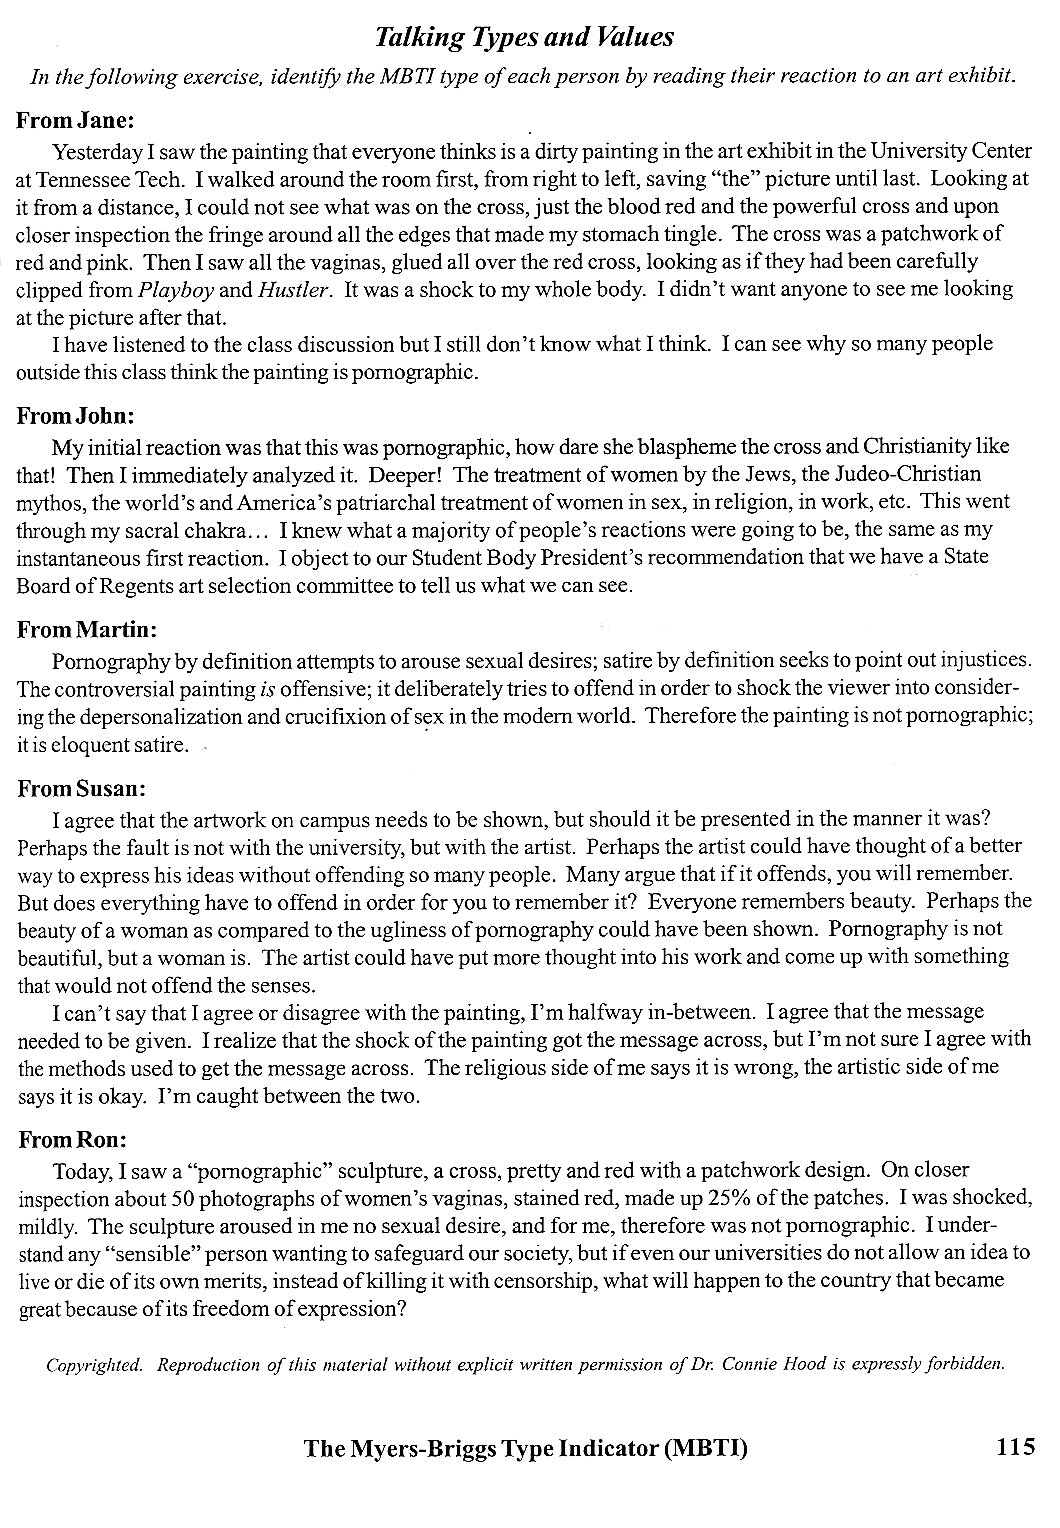
\includegraphics{mbti_test.jpg}}
\end{figure*}

\begin{figure*}[htb]
		\scalebox{0.9}{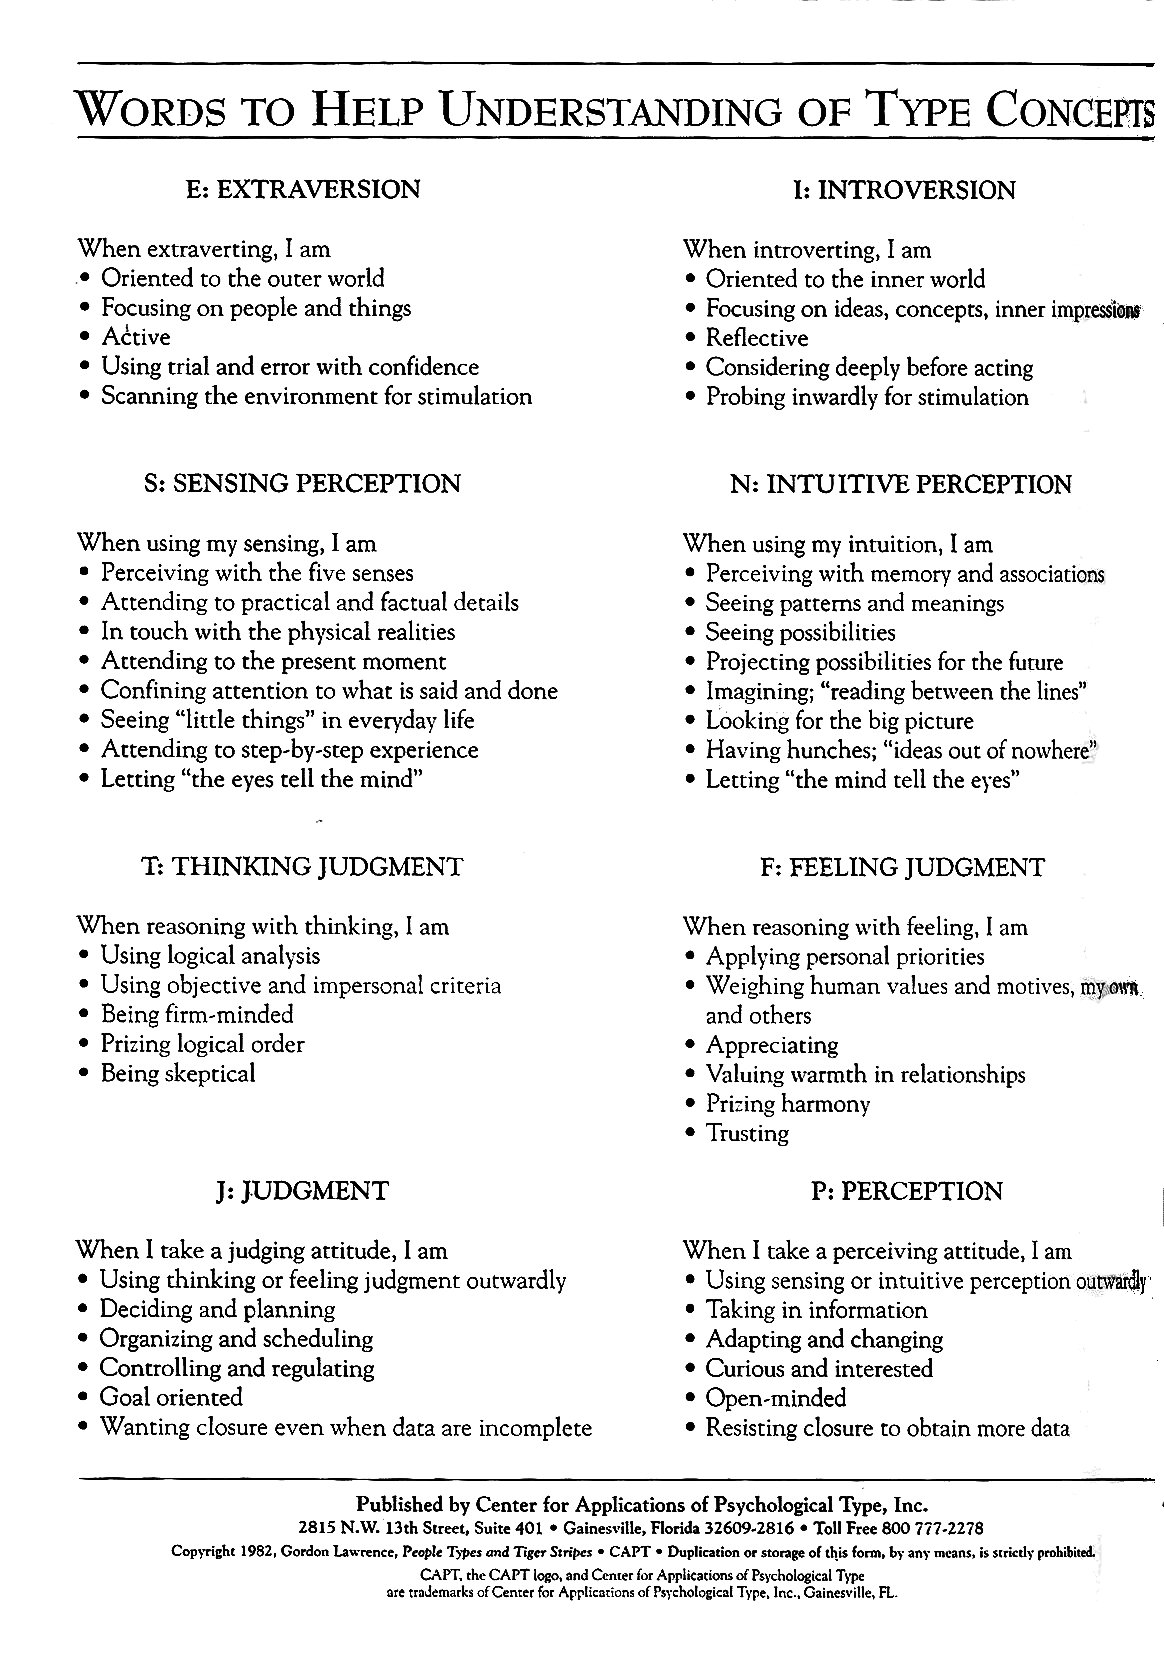
\includegraphics{understanding_type_concepts.jpg}}
\end{figure*}

\begin{figure*}[htb]
		\scalebox{0.8}{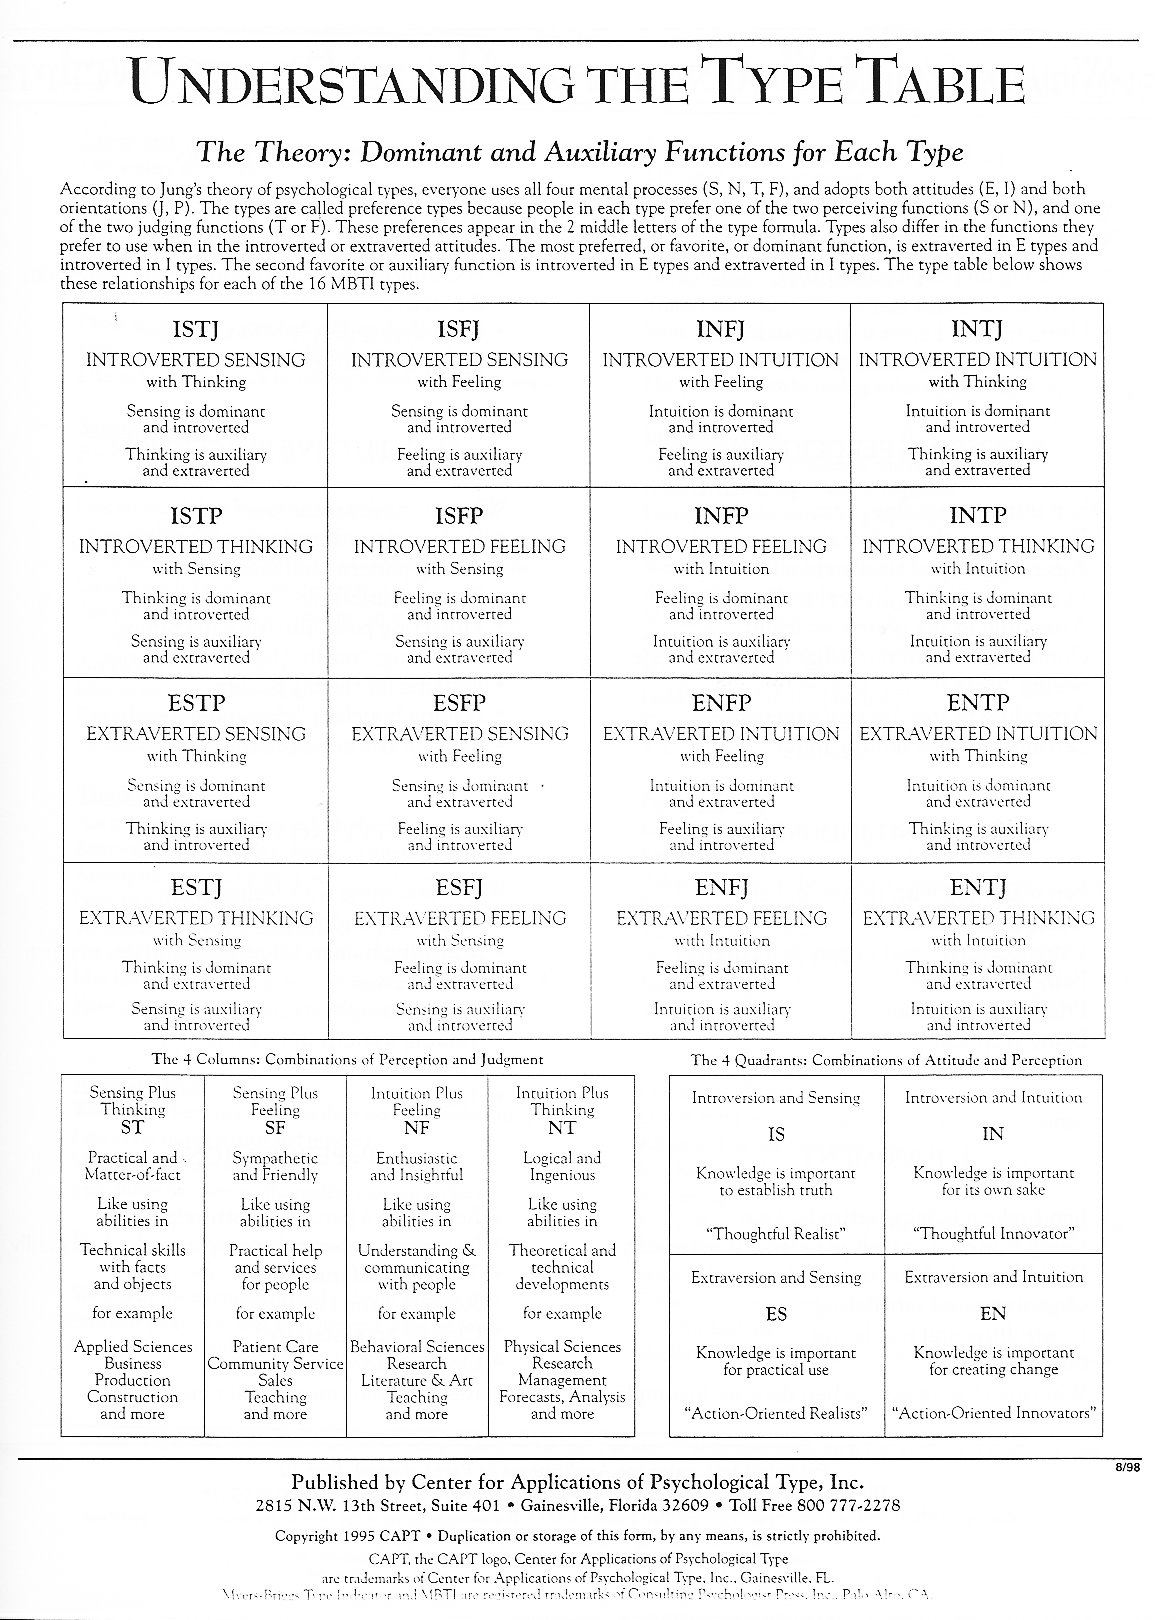
\includegraphics{understanding_type_table.jpg}}
\end{figure*}

\nocite{MBTI:HHB:06,Prov:87,Temp:86,Mar:95,MBTI:HHB:02,chood:87,Jen:95,Kei:98,Law:97,Mic:84,Mye:80}

\bibliographystyle{mla}		% the style you want to use for references.
\bibliography{mr,refs}				% the files containing all the articles and books you ever referenced.
								% MBTI
\chapter{Creating a System of Values (Quinton)}

\begin{authors}
	Quinton Westrich
\end{authors}

\begin{quote}
% Causing an error - wjh 2008/04/14
%	``$\Gamma\nuup\tilde \omegaup\thetaup\iotaup$ $\sigmaup\epsilonup\alphaup\upsilonup\tauup$\~{o}$\nuup$'' \\
	``Gnothi seauton.'' \\
	``Know thyself.''
	\begin{flushright}
		inscribed at the Temple of Apollo at Delphi\footnote{attributed to many Greek philosophers, including Socrates, see ...}
	\end{flushright}
\end{quote}

\section{The Definition of and Case for Values}

\begin{quote}
	"All that we are is a result of what we have thought: it is founded on our thoughts, it is made up of our thoughts."
	\begin{flushright}
		Buddha\footnote{Siddhartha Gautama}
	\end{flushright}
\end{quote}

No action is taken without a preceding thought. Therefore, our actions, in this sense, give us a glimpse, a mirror reflection, of who we are. In examining one's values, we are in essense examining 

There are two definitions of the word \emph{value} which are of relevance here:

\textbf {value} 
1. that quality of a thing according to which it is thought of as being more or less desirable, useful, estimable, important, etc.; worth or the degree of worth 
2. (pl.) the social principles, goals, or standards held or accepted by and individual, class, society, etc.\footnote{citation needed}


$\bullet$ Find moral ambiguities for everyone.

$\bullet$ How do we establish the value of human life?

\section{Some Philosophical Foundations for Moral Values}

\subsection{Relativism}

text

\subsection{Social Contract}

text

\subsection{The Kantian Formalism}

text

\subsection{Utilitarianism}

text

\subsection{Emotivism} %???

text

\section{Roger's Axioms}

\subsection{Radical Honesty}

My commitment to honesty changed more how I communicated to myself than how I communicated to others.

\subsection{Radical Openness}

text

\subsection{Radical Empathy}

text

\subsection{Unconditional Love}

text

\section{Kohlberg's Model of Moral Development}\label{sec:Kohl}

\subsection{Some Context for the Model}

text

\subsection{Stages 1-2: Pre-conventional Levels}

text

\subsubsection{Stage 1: Punishment and Obedience Orientation: Heteronomous Morality}

Heteronomous: subject to external or foreign laws or domination; not autonomous \footnote{(www.dictionary.com) (american heritage dictionary)}

\subsubsection{Stage 2: Individualism, Instrumental Purpose, and Exchange}

text

\subsection{Stages 3-4: Conventional Levels}

text

\subsubsection{Stage 3: Mutual Interpersonal Expectations, Relationships, and Interpersonal Conformity}

text

\subsubsection{Stage 4: Social System and Conscience}

text

\subsection{Stages 5-6: Post-conventional, Principled, or Autonomous Levels}

text

\subsubsection{Stage 5: Social Contract or Utility and Individual Rights}

text

\subsubsection{Stage 6: Universal Ethical Principles}

\begin{quote}
"Any man's death diminishes me, because I am involved in mankind; and therefore never send to know for whom the bell tolls; it tolls for thee\ldots"
\begin{flushright}
John Donne\footnote{\cite{DONNE:1624}}
\end{flushright}
\end{quote}

text

\subsubsection{Stage 7: A Hypothetical Soft Stage}

text

\section{Gilligan}

text

\section{Thic Naht Hanh's 14 Precepts (Andrew Schnell)}

include an introduction

\section{Quotes}

\section{Works Cited}

\section{Further Reading}

text

\bibliographystyle{mla}		% the style you want to use for references.
\bibliography{mr,refs}				% the files containing all the articles and books you ever referenced.
							% Creating a System of Values
\chapter{Models of Development (Avery, Luc, Craig, Quinton)}

\begin{authors}
	Avery Edwards, Luc Robinson, \\ \rule{0.5cm}{0cm} Craig Schuff, and Quinton Westrich
\end{authors}

%%%%%%%%%%%%%%%%%%%%%%%%%%%%%%%%%%%%%%%%%%%%%%%%%%%%%%%%%%%%%%%%%%%%%%%%%%%%%%%%%%%%%%%%%%%%%%%%%%%%%%%%%%%%%%%%

\section{\mbox{Motivational Development:} Maslow's Hierarchy of Needs}

%%%%%%%%%%%%%%%%%%%%%%%%%%%%%%%%%%%%%%%%%%%%%%%%%%%%%%%%%%%%%%%%%%%%%%%%%%%%%%%%%%%%%%%%%%%%%%%%%%%%%%%%%%%%%%%%

\subsection{Levels 1-6: Deficiency Needs}

text

\subsubsection{Level 1: Physiological Needs}

text

\subsubsection{Level 2: Safety Needs}

text

\subsubsection{Level 3: Love/Belonging/Social Needs}

text

\subsubsection{Level 4: Esteem Needs}

text

\subsubsection{Level 5: Cognitive Needs}

text

\subsubsection{Level 6: Aesthetic Needs}

text

\subsection{Level 7: Growth Needs}

text

\subsubsection{Level 7: Self-actualization}

text

%%%%%%%%%%%%%%%%%%%%%%%%%%%%%%%%%%%%%%%%%%%%%%%%%%%%%%%%%%%%%%%%%%%%%%%%%%%%%%%%%%%%%%%%%%%%%%%%%%%%%%%%%%%%%%%%

\section{Cognitive and Ethical Development: Perry's Model}

%%%%%%%%%%%%%%%%%%%%%%%%%%%%%%%%%%%%%%%%%%%%%%%%%%%%%%%%%%%%%%%%%%%%%%%%%%%%%%%%%%%%%%%%%%%%%%%%%%%%%%%%%%%%%%%%

\subsection{Context for the Model}
                                             
In 196? William Perry released the first version of his model of cognitive and ethical growth.  With a  sample of Harvard men ages 18 to 25, Perry outlined the progression of these students as they interpreted aspects of their lives in increasingly complex ways.  Perry's model shows "the evolving ways of seeing the world, knowledge, and education, values, and oneself" over the course of the students' college years.  The progression from 1 through 9 is linear, each new stage including and transcending the previous ones.  This model represents a seminal work in the developmental psychology of young adults.  Following Perry's initial findings researchers have further defined and categorized the development of identity and judgment, but Perry's model serves as a baseline for understanding the process as a whole.

\subsection{Stages 1-3: Dualism Modified}

text

\subsubsection{Stage 1: Basic Duality}

A developmental stage where truth and reality is entirely defined by an authority.  Actions and thoughts are divided into right and wrong, two mutually exclusive categories.  Reasoning at this level commonly is demonstrated by parents looking out for the safety of their children.  At young ages crossing the street is wrong as is touching the stove.  The concepts of "dangerous" or "hot" remain too complex and so action is justified or forbidden solely as an arbitrary declaration of the external authority.  

Stage 2 follows quickly after stage 1
"Of course, doesn't everybody?" often marks the introduction of opposing view points backed by other sources of authority. 

\subsubsection{Stage 2: Multiplicity Prelegitimate}

In this stage of reasoning binary categories continue to be the primary way of labeling sets of ideas and actions.  It is inevitable that a human will encounter others who do not think in the same way given the barest of diversity.  However, in Perry 2 anything not a direct product of the chosen authority is wrong, and broader reasoning as seen in later stages is discounted as logically fallacious.  In the face of differing opinions the correct answers are repeated with a citation of the external authority, case closed.  Students in strictly dualist communities may aspire to leadership positions by memorizing the right rules and parroting them back.  If they know and follow the community guide lines well enough then the ascension into the authority position is a sure thing.  Sense of self and identity are often described in relation to the status quo in position and quality. Statements such as "I am a good student," and "I am not as good a student as a should be," are commonplace at this level of reasoning.

"Even the teacher didn't know the answer!"

\subsubsection{Stage 3: Multiplicity Legitimate but Subordinate}

In Perry 3 diversity of thought is seen as unavoidable for the present time.  Even if truth is not clear now, the authorities are working on the problem and will provide the correct answers as they learn them.  In tightly wound Perry 3 hierarchies the exchange of outside opinions and ideas may be labeled as dangerous or corrupting.  Nonmembers may be demonized to discourage interaction or considered thought between the "right" group and the "wrong" group.  This serves to continually polarize groups of people who devalue mutual understanding and compromise.

"What can we really know?"
Following the recognition of present uncertainty is the realization that uncertainty permeates the whole of human knowledge and experience.  Uncertainty is no longer a temporary state but rather an inherent part of being human.  Depending on personality and background Perry 3 moves into 4a or 4b.

\subsection{Stages 4-6: Relativism Discovered}

text

\subsubsection{Stage 4a: Multiplicity (Diversity and Uncertainty) Coordinate}


4. a) Multiplicity (Diversity and Uncertainty) Coordinate with the "known"
In those who come from an authoritarian background the move into Perry four may be accompanied by shock and bitterness towards former authority figures.  It may be seen as a betrayal to have been taught that everything is certain, when it is discovered that everything is not certain or perhaps even nothing is certain.  This distrust may then be extended onto all sources of authority who sound appear to everything figured out.  If all views contain uncertainty, then by what right can anything be taught as correct or true.  As a reconciliation between a new appreciation for diversity and "common sense" rights, a split system  of dualism and multiplicity.  Contained within the dualist right and wrong category are universal human rights as well as those things considered common sense (regardless of actual population percentage that agrees).  Contrary to early dualism, exchange of opinions on proper action and interpretation of these rights is acceptable.  The second category of belief at this stage is all those things shrouded by reasonable uncertainty.  Ideas, beliefs, and ways of life that do not conflict with the human rights of others are given equal value, with no one system held above another.    Valuation of one opinion above another is seen as an arbitrary judgment, and either dismissed or met with indignation.

\subsubsection{Stage 4b: Relativism Subordinate}

4.b)  Relativism Subordinate
For students who have been encouraged to explore uncertainty by their authority figures, Perry 4b is a common next step.  Perry calls the continued trust for authority adherence.   Subordination in this stage  is characterized by deferral to perceived experience and demonstrated wisdom rather than appeal to position.  Even if an authority figure does not know an answer, the relationship may still yield new ways to approach a concept.  This stage marks the beginnings of internalized or personal authority.  Relativism recognizes that some ideas may be more right than others.  Ideas can now be examined within specific context with relevant logic and evidence rather than tackled as universal absolutes.  Ideas are rejected while others are elevated based on individual merit.  Reasonable people may even disagree on particular ideas without personal animosity.  

\subsubsection{Stage 5: Relativism}

\subsubsection{Journal: Craig Schuff, 26 August 2007}

	\begin{quote}"you know, the anger we have for each other is really meaningless. I'm
 tired of carrying this weight around for nothing. Why don't we just drop the
 anger? It's pointless." \\
 Then as a spur of the moment thing, I called up the stairs to their room,
 saying hi, whussup, and would Kent like to come to Cookeville to eat at
 Beethovin's Bistro?
	\end{quote}


You saw the anger in both of you , then saw your part in keeping it alive,
and then did what was needed to change it (name it, claim it, tame it).
Simply Beautiful Scott.

	\begin{quote}
		Yet there is a difference between knowing about it and being there. And
		really you can't know about it without being there.
	\end{quote}

It always turns out somewhat different than we thought, doesn't it?  From
the inside of a place we have a different view as much as we would like to
think we can understand completely from the outside looking in.  On the
first day of Brit Lit Connie likes to say "Be a little humble about what you
think you know."  I have never received better advice than that.

	\begin{quote}
But what was I doing if I wasn't working through Perry 5? I most certainly
 cared about what I was thinking about, not like Perry 5 at all.  Yet I'm not
 saying anything about how "oh, my god. No absolutes to the universe."
	\end{quote}
	
 I think Perry has never really been an all inclusive description of our
work.  It is possible to work on a huge range of concepts from any point on
Perry.  Morality, Divinity, Reality, all of these things.  Perry is a
measure of how much you externalize this process.  So while it doesn't
affect what you think about, it says a little bit about the manner in which
you think and process.  Also caring about how you think is a first step not
a last step, take heart!

Coming into Perry 5 without a context for it or thought for the other side
can make it suck, but you have spent plenty of time playing with a larger
picture.  This can ease the process significantly, taking universal for all
time wtf angst and making it a personal for now feeling.  This is why we
teach Perry!! Huzzah!!


\begin{quote}
 My Perry 5 is when I accepted the meaninglessness and stopped caring,
 period.
\end{quote}

You spent a good deal of time with it all figured out,  a concept of Perry
down to the last detail.  You cared about this picture, you loved it, and
you wanted it to be perfect.  When you let go of that attachment you were
free to just be where you needed to be.  It is freeing and terrifying.  The
future is uncertain when we let ourselves float along down the river but the
alternative is clinging to our stones, in which case we will certainly sink.


We have been rooting for you, Scott.

Fare Forward Traveler,
Craig

\subsubsection{Stage 6: Commitment Forseen}

text

\subsection{Stages 7-9: Commitments in Relativism Developed}

text

\subsubsection{Stage 7: Commitment}

7.Commitment Made (Single)

\subsubsection{Stage 8: Challenges to Commitment}

8.Commitment Cascade

\subsubsection{Stage 9: Evolving Commitment}

9.Relativism Matured

\subsection{Remarks on the Model}

-Core beliefs
-Regressions
	-alienation
	-Retreat to dualism where differences and complexity can be hated
	-Temporizing

\subsection{Alternative Models of Cognitive Development}

\subsubsection{Baxter Magolda's Model}

1992: cognitive development and learning

\subsubsection{King's and Kitchener's Model}

1994: reflective judgment

\subsubsection{Kohlberg's Model}

1969: cognitive and moral development. see p.\pageref{sec:Kohl}

%%%%%%%%%%%%%%%%%%%%%%%%%%%%%%%%%%%%%%%%%%%%%%%%%%%%%%%%%%%%%%%%%%%%%%%%%%%%%%%%%%%%%%%%%%%%%%%%%%%%%%%%%%%%%%%%

\section{Faith and Spiritual Development}

%%%%%%%%%%%%%%%%%%%%%%%%%%%%%%%%%%%%%%%%%%%%%%%%%%%%%%%%%%%%%%%%%%%%%%%%%%%%%%%%%%%%%%%%%%%%%%%%%%%%%%%%%%%%%%%%

\subsection{Fowler's Model of Faith Development}

\subsubsection{Context for the Model}

-James Fowler backgound

      -prof of theology and human development @ Emory in Atlanta

      -great developmental theorists and researchers of our day, work gaining recognition (jacket cover flap) 

\subsubsection{Stage 1: Primal Faith}

infant, birth is trauma, Tillich's "ontological anxiety," 1st symbols of faith: memories of maternal and paternal presence

\subsubsection{Stage 1a: Incorporative Self}

text

\subsubsection{Stage 2: Intuitive-Projective Faith}

about age 2, language emerges, child questions everything, much novelty and newness, free of preformed constructions, pg. 54: "Perception, feelings, and imaginative fantasy make up children's principal ways of knowing---and transforming---their experiences$\ldots$ For now, stimulated by experience and by stories, symbols, and examples, children form deep and longing-lasting images that hold together their worlds of meaning and wonder." , awakening to mystery of death,

\subsubsection{Stage 2a: Impulsive Self}

text

\subsubsection{Stage 3: Mythic Literal Faith}

around 6 or 7 years, relates to development of Piaget's concrete-operational thinking, pg: 55 "stable categories of space, time, and causality make the child's constructions of experience much less dependent on feeling and fantasy.", child becomes more linear, orderly, and predictable, sense of fairness based on reciprocity, faith becomes matter of reliance on stories, rules, implicit values of the family's community of meanings, narrative/story important, people defined by their affiliations and actions, this stage and the rest can typify adults as well

\subsubsection{Stage 3a: Imperial Self}

text

\subsubsection{Stage 4: Synthetic-Conventional Faith}

usually early adolescence, mind takes wings/formal operational thinking, thinking begins to construct ideal possibilities and hypotheticals, imagination, abstract concepts and ideals, systems, able to construc perspectives of others on ourselves, "mutual interpersonal perspective taking"-accounts for "self-consciousness," pulling together of elements, conventional synthesis of elements gotten from one's significant others, one is embedded in his or her faith outlook, which is tacitly held, deeply felt, but mostly unexamined.

\subsubsection{Stage 4a: Interpersonal Self}

text

\subsubsection{Stage 5: Individuative-Reflective Faith}

shift in sense of grounding and orientation of self, emergence of executive ego (behind the personae/masks), objectification and criticial choosing of beliefs/values/commitments

\subsubsection{Stage 5a: Institutional Self}

text

\subsubsection{Stage 6: Conjunctive Faith}

text

\subsubsection{Stage 6a: Inter-Individual Self}

text

\subsubsection{Stage 7: Universalizing Faith}

text

\subsubsection{Stage 7a: God-Grounded Self}

text

\subsection{A Zen Model of Spiritual Development: The Oxherding Pictures}

\subsubsection{Context for the Model}

text

\subsubsection{Stage 1: Undisciplined}

text

\subsubsection{Stage 2: Discipline Begun}

text

\subsubsection{Stage 3: In Harness}

text

\subsubsection{Stage 4: Faced Round}

text

\subsubsection{Stage 5: Tamed}

text

\subsubsection{Stage 6: Unimpeded}

text

\subsubsection{Stage 7: Laissez Faire}

text

\subsubsection{Stage 8: All Forgotten}

text

\subsubsection{Stage 9: The Solitary Moon}

text

\subsubsection{Stage 10: Both Vanished}

text

\section{Connection and Interplay Among the Developmental Models}

text
\section{Quotes}

\section{Works Cited}

%%%%%%%%%%%%%%%%%%%%%%%%%%%%%%%%%%%%%%%%%%%%%%%%%%%%%%%%%%%%%%%%%%%%%%%%%%%%%%%%%%%%%%%%%%%%%%%%%%%%%%%%%%%%%%%%

\section{Further Reading}

%%%%%%%%%%%%%%%%%%%%%%%%%%%%%%%%%%%%%%%%%%%%%%%%%%%%%%%%%%%%%%%%%%%%%%%%%%%%%%%%%%%%%%%%%%%%%%%%%%%%%%%%%%%%%%%%

The original works by Perry are \cite{Per:70} and \cite{Per:81}. \cite{Per:81} gives the revised version of the model which is contained in this chapter. Other models of development include $\ldots$.

The original works by Fowler are \cite{Fow:84} and \cite{Fow:95}.


\bibliographystyle{mla}		% the style you want to use for references.
\bibliography{mr,refs}				% the files containing all the articles and books you ever referenced.
							% Models of Development
\chapter{Critical Thinking (Quinton, Eamon)}

\begin{authors}
	Eamon Ryan and Quinton Westrich
\end{authors}

\section{Introduction}

If you're reading this chapter, I think it's safe for me to assume that you have decided to examine yourself and your conception of the world at a deeper level than the \emph{hoi polloi}\index{hoi polloi}, i.e.\ the common man. No doubt, not everyone chooses this path-- what Robert Frost called "the road less traveled." Should the road prove a bit bumpy (often a good sign, a precursor to self-transformation!) we should develop some tools to aid our journey. 

When I started Mentor, I had already spent a few years reading and thinking about philosophical questions. I was eager to join a group of intellectuals in a search for deeper truths. However, I was deeply bothered by the seemingly incessant assumption that there were flaws in my thinking, or that I was somehow a beginner in the search for truth. Grudgingly, I traveled forward, disdainfully examining things I had already "figured out" to humor Dr.\ Hood or to prove the assumption vacuous. 

I can now admit that my reasoning is still loaded with faulty assumptions and poor logic. However, it's a whole world clearer than it was to begin with! And the thought of having an idea "figured out" seems quite presumptuous to me now. My experience has suggested to me that new data will often emerge and force me to change my current beliefs if I wish to remain honest and accurate with my observations. In this sense, humility is not something which only virtuous people have, but something which arises out of necessity and awareness.

Each year, Dr.\ Hood included in her introductory speech to incoming Honors freshman a bit of advice: "Be a little humble about what you \emph{think} you know." Now I realize she wasn't talking down to us as I had first interpreted. She was sharing her wisdom about a way of being. It was not intended solely for freshmen, but as a piece of advice to live with and hold even as we become upper-classmen, graduate students, and professionals. 

With that said, this chapter is essentially about learning how to think. The assumption is that you're probably not exactly right about everything 100\% of the time. Notwithstanding, we proceed with hope of at least improving our attempts at seeking awareness. We'll introduce some tools for making our ideas clear, keeping our reasoning sound, and keeping ourselves honest. The tools include an awareness of both a collection of examples of pseudoreasoning, or \emph{logical fallacies}, and common ways our emotions cloud our judgments, or \emph{defense mechanisms}.

These tools are also useful for evaluating the utility and validity of arguments presented by others. If we each had to figure \emph{everything} out for ourselves, it would take 10 years to just establish that $1+1=2$ \cite{WhRu:62}! In order to speed up the process, we can read the works of others and listen to their arguments \emph{critically}, accepting what we see as likely, reasonable, or attractive and rejecting what we see as unlikely, unreasonable, or repulsive. While all this is good in theory, we cite a journal below of what one mentor student experiences in reality.

\subsubsection{Journal: Eric Hoy, 29 June 2007}

\begin{quotation}
Well I'm back at home and still slightly irritated from the car trip. I hate watching my parents do the same things I do. Especially when I don't like those things such as over-criticism, narrow-mindedness, and the "win" the argument mentality. I realized another reason that I don't like to be criticized or appear at a loss for words. In my family (especially with my dad), silence and loss of words is taken as having "lost" the argument. I noticed this dynamic as I was talking with my dad. I was very tired today and in an argumentative mood so I saw how I can argue. I can contradict myself 10 or 20 times in an argument. I don't get the facts straight once the discussion gets heated. I noticed my dad uses name calling to derail one's argument (calling me a "liberal," "stuck up," or "self-centered" as if being these ruin my argument). I have fallen into this logical fallacy many times when I feel backed into a corner (like him), but never to the extent he does. Saying the "wrong" thing ends the discussion. He treats the arguments like games (another trap for me). I don't think they're so fun anymore. It is his way of interaction (and it drives my mom up the wall sometimes). I do see the two in one mind when they are criticizing the stupidity or recklessness of others (guess where my complexes with security and competence come from, I just realized this). Again this irritated me greatly, another hole I can fall into, over-criticizing. Basically these issues could be summed up as security issues to me. Ways of defending one's competence and beliefs. Being my parents for so long is not as bad as I think it is.

Erik
\end{quotation}


\section{What is critical thinking?}

\subsection{Claims, Meaning, and Truth}

In this section, we'll present some definitions and motivation for pursuing our as-of-yet undefined term "critical thinking." Let us remedy the undefinedness; but, first, we need a leading definition: A \bigwerd{claim} is a statement for which the labels `true' and `false' make gramatical sense. So, not everything that is said is a claim: interogative, exclamatory, and imperative statements are excluded, while declarative statements are generally included. The common purpose of a claim is \emph{to communicate information}. However, this purpose is not usually realized in actual conversation. Humans often engage in sarcasm, small talk, and generally non-informative communication to keep a balance of human needs; we are emotional as well as reasoning creatures. Thus it has become quite tricky to spot a claim. Often we mistake witty comments for claims.

We stop here to remark about the words `true\index{true}' and `false' used above. While the definition given, is often valid, we might come across cases in which we have a claim which defies this characterization. For example, Heraclitus's statement "The way up is the way down," and many Zen koans fit this latter category of claims. These are the subject of Chapter \ref{ch:paradox}, which discusses \bigword{paradox}. In our definition, we allow the case in which a claim is claimed to be \bigword{both true and false} or \bigword{somewhat true} or \emph{somewhat false}. Often these cases can be resolved into a classification of \bigword{relatively true} or \emph{relatively false} with a change in context.

For example, you might say "Rainy weather is depressing." What does this \emph{mean}?\footnote{Admitedly, such an analysis of this particular statement is ridiculous. However, I thought it a neutral example, suitable for demonstration purposes. Nontrivial examples will be cited later.} This leads us to our next caveat: Meaning only exists within some context. This you can verify by experiment. In our example, the \emph{implicit} context is that of the emotional state of all humans, that is, all humans feel depressed whenever it is raining in that particular human's location.

\subsection{Critical Thinking, Dialogue, and Dialectic}

\textbf{Critical thinking}\index{critical thinking} is the careful, deliberate determination of whether we should accept, reject, or suspend judgment about a claim---and of the degree of confidence with which we accept or reject it.

\subsubsection{dialectical}
noun - The art or practice of arriving at the truth by the exchange of logical arguments.
The process especially associated with Hegel of arriving at the truth by stating a thesis, developing a contradictory antithesis, and combining and resolving them into a coherent synthesis.
\subsubsection{sophists}
noun - One skilled in elaborate and devious argumentation. A scholar or thinker.
Sophist Any of a group of professional fifth-century B.C. Greek philosophers and teachers who speculated on theology, metaphysics, and the sciences, and who were later characterized by Plato as superficial manipulators of rhetoric and dialectic.
\subsubsection{didactical}
adjective - intended for instruction; instructive: didactic poetry.
inclined to teach or lecture others too much: a boring, didactic speaker.	teaching or intending to teach a moral lesson. didactics, (used with a singular verb) the art or science of teaching.
adj.Intended to instruct. Morally instructive. Inclined to teach or moralize excessively.

\section{Some Common Logical Fallacies and Pseudoreasoning}

Logical fallacies and pseudoreasoning enrich our lives in ways we might never have anticipated...

\subsubsection{Non Sequitor}
Latin for "it does not follow," ask yourself "Does this logically connect?" In order to be clear in our arguement or discussion, our thought progression should be linked together. 

\subsubsection{Overgeneralization}
Qualifying and asserting a claim as an absolute and not addressing other existing possibities, i.e. asserting a claim holds in a larger context because it applied to a previous specific context.

\subsubsection{Oversimplification}
Simplifying a definition may be usefull while under a constraint of time but with specific language orientation and also scientific processes, breaking down an arguement could create ambiguity in a discussion, debate, or writing. Oversimplication is a very important concept to remember especially when considering language use in dialectical reasoning.

\subsubsection{Post hoc, ergo propter hoc}
Latin for "after this, therefore because of this?." Events sometimes occur in a successive fashion but do not necessarily become an explicit part of reasoning for another event.

\subsubsection{Red herring}
This could also be referred to in mentor terminology as "Bouncing." Example - Having a conversation about G.W. Bush and then talking about Al Gore's sons' arrest for marijuana.

\subsubsection{Reificaiton}

\subsubsection{Relativist fallacy}

\subsubsection{Resorting to Clich\'e}
Using a popular phrase or expression to summate an action or dialectical arguement.

\subsubsection{Sequential fallacy}
reference to check on if different then post hoc ergo propter hoc house of quinton

\subsubsection{Slippery slope}

\subsubsection{Slothful principle}

\subsubsection{Spotlight}

\subsubsection{Straw man}

\subsubsection{Style over substances}
Looks over content.

\subsubsection{Two wrongs make a right}

\subsubsection{Unevaluated contingency}


\section{Defense Mechanisms}

\begin{quote}
	"Anything outside yourself, this you can see and apply your logic to it$\ldots$ but it's a human trait that when we encounter personal problems, those things most deeply personal are most difficult to bring out for our logic to scan. We tend to flounder around, blaming everything but the actual, deep-seated thing that's really chewing on us."
	\begin{flushright}
		in \emph{Dune}
	\end{flushright}
\end{quote}


\subsubsection{Assimilation}

\subsubsection{Denial}

\subsubsection{Displacement}

\subsubsection{Externalization}

\subsubsection{Projection}

\subsubsection{Rationalization}

\subsubsection{Reaction formation}

\section{An Application to Ethics}
\subsection{Ethos, Logos, and Pathos}
\subsection{What is Rhetoric?}
\subsection{What is a Syllogism?}

\section{Clarity...}

\section{Quotes}

\section{Works Cited}


\section{Further Reading}

A full onslaught into the subject of critical thinking can be found in any number of standard texts often used in university philosophy courses. One which has been used as a reference herein is \cite{MoPa:01}. We've also pulled material from the Tennessee Tech \emph{Honors Handbook} \cite{Hon:06} and \emph{Thinking Critically About Ethical Issues} \cite{Ru:04}.

\bibliographystyle{mla}		% the style you want to use for references.
\bibliography{mr,refs}				% the files containing all the articles and books you ever referenced.
		% Critical Thinking
\chapter{Mindfulness (Craig)}

\begin{authors}
	Craig Schuff
\end{authors}

\section{Introduction}

Definition of Mindfulness\index{mindfulness}:
\begin{enumerate}
	\item Observing in the present moment
	\item Leaving off judgment
\end{enumerate}

\section{Noticing}

\begin{enumerate}
	\item What we do not notice still occurs
	\item When we notice we can then act on this thing as it has been acting on us
\end{enumerate}

\section{Naming}

\begin{enumerate}
	\item After noticing something new we seek to attach a name to it.  What is this new thing?
	\item The names we give identify what we are doing in the simplest terms available
	\item If a better name becomes apparent then use it
	\item Naming will greatly improve our practice of noticing. 
\end{enumerate}

\section{Patterns}

\begin{enumerate}
	\item With a little time spent noticing and naming we start to see things repeating.
	\item This is in itself something new to notice.  "I have done this before!"
\end{enumerate}

\section{Mindfulness Practices}

\begin{enumerate}
	\item Mindfulness: Observing in the present moment
	\item Practice:  You get better at it!
\end{enumerate}

\subsection{Senses}

Notice and name your senses. 

Sight

Sound

Touch

Smell

Taste 

Part 1 

Start with an experience.  Leaves in the fall for example. 

As you experience a sensation pull out the part that is sight.  Explore that sensation.  Roll it around in your mind while repeating "Sight... Sight... Sight," in your head. 

Pull out the sound.  Explore it.  Leaves rustling "Sound... Sound... Sound." 

Pull out the touch.  Wind blowing.  Wind in hair.  Air over skin.  Chill.  Watering eyes.   "Touch... Touch... Touch" 

Pull out the smell.   

Pull out the taste 

Not every experience will involve strong sensations in every category.  No need to create what is not there.  Now, if the experience involved apple pie, ah! 

Part 2 

Leaves again 

Within an experience take each sense again.  This time name what other sensations directly interact with this one. 

"Sight... Sight... Sight"

The feeling of my eyes during sight "Touch" 

"Sound... Sound"

Feeling my ears during sound "Touch"

Feeling sharp sound on my ears "Touch"

Feeling a loud low sound on my body "Touch" 
 

Wind on my face "Touch"

Wind moving the leaves "Sight"

Pressure in my ears "Touch"

crunching noise "Sound"

Person walking through leaves "Sight"

\subsection{Colors}

First pick a color.  Everywhere you go notice this color.  When you see your color say it in your mind.  "Red"... "Red"... "Red."  Do this whatever else you are doing, where ever you are.  During conversations, during lectures, while walking, while writing notice your color and say it in your mind.  
 
Doing this for any length of time is where discipline comes in.  You will be distracted, you will forget to notice your color despite all of your best intentions.  When you notice that you are not doing the exercise recognize it and start again.  
 
Wear a rubber band on your wrist.  You will find often that you have forgotten to see your color.  The rubber band will help remind you.  It is easy to go days without remembering color, it is harder to miss a rubber band on your wrist.  
 
Each day you may pick a new color to notice.  Choose something other than black or white. 
 
 
 
Journal during this experience.   
What do you notice?   
What do you notice yourself doing? 
Does the experience change at all?  Is it different thinking "Red" after 20 minutes than it is after 6 hours?  
Is it easy to remember? 
Is it difficult to do something as simple as naming a color for very long? 
Do you become Frustrated?  Tired?  Bored?  Elated? 
Notice yourself in relationship to this discipline. 
 
 
You do not need to write all of your journal in one sitting.  Write what you notice even if it is only one thought, one sentence, one word.  If you notice more the next day then add more.

\section{Quotes}

\section{Works Cited}

\section{Further Reading}

\bibliographystyle{mla}		% the style you want to use for references.
\bibliography{mr,refs}				% the files containing all the articles and books you ever referenced.
					% Mindfulness
\chapter{Wisdom (Jon)}

\begin{authors}
	Jon Jones
\end{authors}

\section{What is Wisdom?}

\begin{quote}
Where is the Life we have lost in living?\\
Where is the wisdom we have lost in knowledge?\\
Where is the knowledge we have lost in information?"\\
\begin{flushright}
	T.S. Eliot
\end{flushright}
\end{quote}

What is wisdom? What does the word "wisdom" mean? Where are the wise sages and their teachings? To many, wisdom is an indefinable yet invaluable quality that seems to be just beyond succinct description. Some note psychologists, such as Dr. Robert Sternberg and others, have said that one needs a certain level of wisdom to identify and understand wisdom. Furthermore, some believe there is a prerequisite level of knowledge or intelligence needed either to decode the meaning of a wise assertion or to see the potential wisdom in a statement. Can wisdom be taught? The answer may at best be, yes and no. It is perhaps more easily conveyed through an analogy about a well kept and robust garden. In the Garden of wisdom there are kernels of insight and seeds of knowledge. The water could be considered as experience and the soil as the mind with its intelligence and predisposition to novelty. Lastly, we could imagine the sun as patience and think of it as representing the cyclic nature of many aspects of personal growth.

However, we've still not reached a true definition or even understanding of the many meanings and manifestations of wisdom. The analogy is reasonable for starting out, but there is a form of wisdom in knowing the boundaries between multidimensional reality and multifaceted symbolism / metaphor. Is wisdom a way of thinking? Is it a way or method of reasoning, discerning, decision making, or structuring thoughts? Is it the way one prioritizes aspects or actions according to some moral or ethical principle? Is it a way of knowing, objectively or subjectively, the truest nature of things? Is it a way of knowing the most efficient or most practical things and courses of action? Is wisdom the aggregate accretion of esoteric knowledge or truth, long ago discovered and closely guarded? Is wisdom a way of being? Is it a state of being? Is it a state of mind or a state of development? Is it part of a larger process of development? Is it the final stage or the beginning of a whole other paradigm and ontology? Is all wisdom created equal? Is it all the same wisdom or are there many kinds of wisdom?

The word "wisdom" is very much like many other English words in that it is composed of letters, has an etymology,   has separate definitions depending on context, and is a referent (not the thing itself but a symbolic representation of the thing. As a word and a concept, wisdom and its variety of meanings is subject to change. If one wants to solve a mystery, they follow the clues. If one wants to define wisdom, then one must follow the word in its denotations and connotations through the ages. Above all else, the most important aspect of the search must be context. Definitions come from specific contexts, and hence the OED's incredibly large etymologies. Wisdom is perhaps also analogous to a tree, having large dendrite-like branchings fanning out according to time, place, meaning, and use.

As we track wisdom through the ages we see a move from a single wisdom into a more diversified pair that expand upon the original grouping of knowledge, sayings, beliefs, and prudent actions held together under the banner of "good" (if not best) things to do and ways to live). There are then two main branches of wisdom in the ancient societies beginning about 5,000 BCE. These branches are what I call Practical Wisdom and Divine Wisdom. The delineation is as follows.
 
[insert citations and proff of what I'm saying]
 
Practical wisdom came to encompass and perhaps spur the development of such ideas and structures as cultural conventions, societal beliefs about the way the world worked, conventional wisdom about society and environment. Divine wisdom, on the other hand, seems to have been integrated with if not developed out of the teachings of early religion and mythology. Such things as truth from religions revelation, transcendental experiences, paradoxical observations, mystical meanings, and introspective thought in relation to the world and life and death seem to have all come from a related set of experience and thinking.

We must remember that wisdom is much like a family tree. Wisdom and its associated words belonged to these cultures and were in daily use by the people. It grew and changed with the people as they used these concepts and explored them, creating a more divers spectrum of ideas, heuristics, and ways of acting. Volitional, affective, intellectual. And so, wisdom has come to reflect their beliefs as well as their priorities in the writings that remain.
 
[Insert history of wisdom from anthropology books / handbook on wisdom / 1990 wisdom book / holliday and chandler]
 
[talk about the models]
 
[talk about ways it relates to a path of development]
 
[relate that to mentor]
 
you enrich the ming / soil of the garden with mindfullness trainning.
 
it's not just a werstern conception
 
[Nvak's world's wisdom]
 
 
[ our definitins of wisdom and what we think it means and why its important.]
 
[box]
[square]
[rectangle]
[two equivalent triangles stuck together at the hypotenuse]

\section{Sternberg Stuff (scanned)}


\section{Russell's "Knowledge and Wisdom"}

(We need to truncate this! There's a typo in here somewhere!)

Most people would agree that, although our age far
surpasses all previous ages in knowledge, there has
been no correlative increase in wisdom. But agreement
ceases as soon as we attempt to define `wisdom' and
consider means of promoting it. I want to ask first
what wisdom is, and then what can be done to teach it.
There are, I think, several factors that contribute to
wisdom. Of these I should put first a sense of
proportion: the capacity to take account of all the
important factors in a problem and to attach to each
its due weight. This has become more difficult than it
used to be owing to the extent and complexity of the
specialized knowledge required of various kinds of
technicians. Suppose, for example, that you are
engaged in scientific research in medicine. The work
is difficult and is likely to absorb the whole of your
intellectual energy. You have not time to consider the
effect which your discoveries or inventions may have
outside the field of medicine. You succeed (let us
say), as modern medicine has succeeded, in enormously
lowering the infant death-rate, not only in Europe and
America, but also in Asia and Africa. This has the
entirely unintended result of making the food supply
inadequate and lowering the standard of life in the
most populous parts of the world. To take an even more
spectacular example, which is in everybody's mind at
the present time: You study the composistion of the
atom from a disinterested desire for knowledge, and
incidentally place in the hands of powerful lunatics
the means of destroying the human race. In such ways
the pursuit of knowledge may become harmful unless it
is combined with wisdom; and wisdom in the sense of
comprehensive vision is not necessarily present in
specialists in the pursuit of knowledge.

Comprehensiveness alone, however, is not enough to
constitute wisdom. There must be, also, a certain
awareness of the ends of human life. This may be
illustrated by the study of history. Many eminent
historians have done more harm than good because they
viewed facts through the distorting medium of their
own passions. Hegel had a philosophy of history which
did not suffer from any lack of comprehensiveness,
since it started from the earliest times and continued
into an indefinite future. But the chief lesson of
history which he sought to inculcate was that from the
year 400AD down to his own time; Germany had been the
most important nation and the standard-bearer of
progress in the world. Perhaps one could stretch the
comprehensiveness that contitutes wisdom to include
not only intellect but also feeling. It is by no means
uncommon to find men whose knowledge is wide but whose
feelings are narrow. Such men lack what I call wisdom.

It is not only in public ways, but in private life
equally, that wisdom is needed. It is needed in the
choice of ends to be pursued and in emancipation from
personal prejudice. Even an end which would be
noble to pursue, if it were attainable, may be pursued
unwisely if it is inherently impossible of
achievement. Many men in past ages devoted their lives
to a search for the philosopher's stone and the elixir
of life. No doubt, if they could have found them, they
would have conferred great benefits upon mankind, but
as it was their lives were wasted. To descend to less
heroic matters, consider the case of two men, Mr A and
Mr B, who hate each other and, through mutual hatred,
bring each other to destruction. Suppose you go to
Mr A and say, 'Why do you hate Mr B?' He will no doubt
give you an appalling list of Mr B's vices, partly
true, partly false. And now suppose you go to Mr B. He
will give you an exactly similar list of Mr A's vices
with an equal admixture of truth and falsehood.
Suppose you now come back to Mr A and say, 'You will
be surprised to learn that Mr B says the same things
about you as you say about him', and you go to Mr B
and make a similar speech. The first effect, no doubt,
will be to increase their mutual hatred, since each
will be so horrified by the other's injustice. But
perhaps, if you have sufficient patience and
sufficient persuasiveness, you may succeed in
convincing each that the other has only the normal
share of human wickedness, and that their enmity is
harmful to both. If you can do this, you will have
instilled some fragment of wisdom.

I think the essence of wisdom is emancipation, as far
as possible, from the tyranny of the here and now. We
cannot help the egoism of our senses. Sight, sound
and touch are bound up with our own bodies and cannot
be impersonal. Our emotions start similarly from
ourselves. An infant feels hunger or discomfort, and
is unaffected except by his own physical condition.
Gradually with the years, his horizon widens, and, in
proportion as his thoughts and feelings become less
personal and less concerned with his own physical
states, he achieves growing wisdom. This is of course
a matter of degree. No one can view the world with
complete impartiality; and if anyone could, he would
hardly be able to remain alive. But it is possible to
make a continual approach towards impartiality, on the
one hand, by knowing things somewhat remote in time or
space, and on the other hand, by giving to such things
their due weight in our feelings. It is this approach
towards impartiality that constitutes growth in
wisdom.

Can wisdom in this sense be taught? And, if it can,
should the teaching of it be one of the aims of
education? I should answer both these questions in the
affirmative. We are told on Sundays that we should
love our neighbors as ourselves. On the other six days
of the week, we are exhorted to hate. But you will
remember that the precept was exemplified by saying
that the Samaritan was our neighbor. We no longer
have any wish to hate Samaritans and so we are apt to
miss the point of the parable. If you want to get its
point, you should substitute Communist or
anti-Communist, as the case may be, for Samaritan. It
might be objected that it is right to hate those who
do harm. I do not think so. If you hate them, it is
only too likely that you will become equally harmful;
and it is very unlikely that you will induce them to
abandon their evil ways. Hatred of evil is itself a
kind of bondage to evil. The way out is through
understanding, not through hate. I am not advocating
non-resistance. But I am saying that resistance, if it
is to be effective in preventing the spread of evil,
should be combined with the greatest degree of
understanding and the smallest degree of force that is
compatible with the survival of the good things that
we wish to preserve.

It is commonly urged that a point of view such as I
have been advocating is incompatible with vigour in
action. I do not think history bears out this view.
Queen Elizabeth I in England and Henry IV in France
lived in a world where almost everybody was fanatical,
either on the Protestant or on the Catholic side. Both
remained free from the errors of their time and both,
by remaining free, were beneficent and certainly not
ineffective. Abraham Lincoln conducted a great war
without ever departing from what I have called wisdom.

I have said that in some degree wisdom can be taught.
I think that this teaching should have a larger
intellectual element than has been customary in what
has been thought of as moral instruction. I think that
the disastrous results of hatred and narrow-mindedness
to those who feel them can be pointed out incidentally
in the course of giving knowledge. I do not think that
knowledge and morals ought to be too much separated.
It is true that the kind of specialized knowledge
which is required for various kinds of skill has very
little to do with wisdom. But it should be
supplemented in education by wider surveys calculated
to put it in its place in the total of human
activities. Even the best technicians should also be
good citizens; and when I say 'citizens', I mean
citizens of the world and not of this or that sect or
nation. With every increase of knowledge and skill,
wisdom becomes more necessary, for every such increase
augments our capacity of realizing our purposes, and
therefore augments our capacity for evil, if our
purposes are unwise. The world needs wisdom as it has
never needed it before; and if knowledge continues to
increase, the world will need wisdom in the future
even more than it does now.

\begin{table*}
	\centering
	\begin{tabular}{lp{6cm}}
		\hline\hline
		Author(s) & Definition \\
		\hline
		Robinson	& \emph{Three historical definitions}: \\
							& \emph{Greek:} an intellectual, moral, practical life; a life lived in conformity with truth, beauty \\
							& \emph{Christian:} a life lived in pursuit of the divine, absolute truth \\
							& \emph{Contemporary:} a scientific understanding of laws governing matter in motion	\\
		\hline
		Csikszentmihalyi &	word	\\
		and Rathunde						&		word	\\
		\hline
	\end{tabular}
	\caption{Definitions of Wisdom}
\end{table*}

\begin{flushright}
by Bertrand Russell
\end{flushright}

\section{Quotes}

\section{Works Cited}

\section{Further Reading}


\bibliographystyle{mla}		% the style you want to use for references.
\bibliography{mr,refs}				% the files containing all the articles and books you ever referenced.
							%	Wisdom
\chapter{Readings and Movies (Connie)}

\begin{authors}
	Connie Hood
\end{authors}

\begin{authors}
	people who eventually send me stuff
\end{authors}

words words words




\bibliographystyle{mla}		% the style you want to use for references.
\bibliography{mr,refs}				% the files containing all the articles and books you ever referenced.
						% Readings and Movies
\part{Level 2 Work}
\chapter{Personal Development II (Connie)}

\begin{authors}
	Connie Hood
\end{authors}

\begin{authors}
	people who eventually send me stuff
\end{authors}

words words words


\section{Quotes}

\section{Works Cited}

\section{Further Reading}


\bibliographystyle{mla}		% the style you want to use for references.
\bibliography{mr,refs}				% the files containing all the articles and books you ever referenced.
						% Personal Development 2
\chapter{Community (Connie)}

\begin{authors}
	Connie Hood
\end{authors}

words words words


\section{Quotes}

\section{Works Cited}

\section{Further Reading}


\bibliographystyle{mla}		% the style you want to use for references.
\bibliography{mr,refs}				% the files containing all the articles and books you ever referenced.
						% Community
\chapter{MBTI II (Connie)}

\begin{authors}
	Connie Hood
\end{authors}

\begin{authors}
	people who eventually send me stuff
\end{authors}

words words words


\section{Quotes}

\section{Works Cited}

\section{Further Reading}


\bibliographystyle{mla}		% the style you want to use for references.
\bibliography{mr,refs}				% the files containing all the articles and books you ever referenced.
								% MBTI 2
\chapter{Values II (Connie)}

\begin{authors}
	Connie Hood
\end{authors}


words words words


\section{Quotes}

\section{Works Cited}

\section{Further Reading}


\bibliographystyle{mla}		% the style you want to use for references.
\bibliography{mr,refs}				% the files containing all the articles and books you ever referenced.
							% Values 2
\chapter{Spirituality (Deanna Light)}

\begin{authors}
	Connie Hood
\end{authors}

words words words


\section{Quotes}

\section{Works Cited}

\section{Further Reading}


\bibliographystyle{mla}		% the style you want to use for references.
\bibliography{mr,refs}				% the files containing all the articles and books you ever referenced.
				% Spirituality
\chapter{Mysticism}

\begin{authors}
	by ???
\end{authors}



\section{Underhill's Model}

\subsubsection{Context for the Model}

text

\subsubsection{Stage 1: Awakening}

text

\subsubsection{Stage 2: Purgation}

text

\subsubsection{Stage 3: Illumination}

text

\subsubsection{Stage 4: Dark Night of the Soul}

text

\begin{quotation}
	\hspace{1.5cm}Convergence\\[5pt]
	\noindent I feel my tortured soul begin to rend. \\
	Oh, pity me, that I have left behind \\
	The naked beauty of a newborn mind. \\
	I find it very difficult to bend \\
	Away from roads to which all mortals tend. \\
	For time beyond my portion have I pined, \\
	Though now within my plundered heart I find \\
	A deep and dreadful longing for the end. \\
	For Peace! For Peace! I plead for bless-ed Peace, \\
	That the conducting of this damn-ed dirge \\
	Which is my life might cease! For Peace! For Peace! \\
	Withhold me not from Peace! Completely purge \\
	From me the urge to break apart from Peace! \\
	And then there comes a surge---and I converge. \\
	
	- Neil Cowden
\end{quotation}

\subsubsection{Stage 5: Union}

text
\chapter{Paradox (Connie)} \label{ch:paradox}

\begin{authors}
	by people who eventually send me stuff
\end{authors}

\section{Paradox in Eliot: from Craig}

T.S. Elliot
From Little Gidding

"There are three conditions which often look alike
Yet differ completely, flourish in the same hedgerow:
Attachment to self and to things and to persons, detachment
From self and from things and from persons; and, growing between them,
indifference
Which resembles the others as death resembles life,
Being between two lives�unflowering, between
The live and the dead nettle."

First state:  attachment to self and to things and to persons
Second state: detachment from self and from things and from persons

Resolution: growing between them, indifference
Which resembles the others as death resembles life

The Paradox is the simultaneous realization of the two states which
seemingly exclude each other.  This resolution resembles the original
statements not at all.  The two opposites held in tension creates a
force which is entirely new and unexpected.

\subsubsection{Journal: John Visel, 31 July 2007}

Here's a poem I wrote a two years ago.  In retrospect, it's something
of a baby picture, but many times, I still think this way.  I think I
was trying Rumi's ideas on for size- I didn't really ``know'' them on any
significant level yet, but looking back, it was a growth step to
pretend his ideas were something I embodied.  That sort of thing is the
spiritual equivalent of children playing ``house'' or ``school'' or
``grownups.''  It's part of how we learn in any arena.

John

***

\medskip

\noindent The mystery used to have an answer\\
It was just elusive, and I could never find it.\\
Now, the answer to the mysteries of life\\
are not what I'm seeking as much,\\
More just to develop a relationship with them.\\
The mystery is like a spiritual figure\\
Or a sensual desire, of something\\
we know next to nothing about,\\
only that it's attractive\\
The artists\\
Have this on a personal\\
and spiritual level.\\
Beethoven's Immortal Beloved\\
(not to mention this happening\\
all over spirituality/mysticism.)\\
Someone who is far away, is prescribed\\
godlike status, yet whose foundation\\
or real definition, we don't really know.\\
This happens all over the place\\
Love from Afar\\
Dante's Beatrice,\\
Petrarch's Laura,\\
Bocaccio's Fiammetta,\\
These loves are different than normal ones\\
We know they're not attainable\\
in any earthly form,\\
Yet they're divinely attractive\\
What a tough concept to get one's\\
head around!\\

\medskip

\noindent The reward of this kind of mystery\\
is in the striving for it.\\
To achieve the ``answer'' to this mystery,\\
one must transform.\\
The answer may lie in the person you become\\
once you've struggled with this\\
and it has hurt you\\
in a big-context sort of way.\\

\medskip

\noindent Perhaps we're not looking off in to\\
some faraway place for this love\\
Perhaps we're looking in at the divine\\
or god-part of ourselves.\\
Perhaps that's why we can't find\\
and answer in the form that we want it.\\
Perhaps that's why we so much think\\
That it's just one thing.\\

\medskip

\noindent Much of the pain we've been through\\
has been because we're looking for an answer\\
in a form that we've long since outgrown\\
And when you finally realize this,\\
and learn to just be with the mystery,\\
It doesn't feel like you're getting answers\\
anymore.  Yet you're content.\\
In reality, you've come to terms with the mystery,\\
and that may be the answer itself.\\
In that sense, most of us are barking\\
up the wrong tree,\\
Or climbing a lifelong ladder,\\
Only when we reach the top, tired, and frustrated,\\
We find that we've put our ladder\\
up against the wrong building.\\

\medskip

\noindent Live with the mysteries\\
Myteries are a condition,\\
not a question with an answer.\\
Mysteries are a space in which to put yourself,\\
not a question with an answer.\\

\medskip

\noindent Most of us assume that there is just one answer\\
Which is fascinating. Our minds are instinctively\\
steering us toward one-ness\\
Why must there be just one?\\
Perhaps if we were content with many answers\\
for the same question,\\
it wouldn't be quite so intriguing.\\
And we wouldn't strive\\
quite so hard.\\
The striving, after all, I think,\\
is how we progress down this path.

\section{Quotes}

\section{Works Cited}

\section{Further Reading}

\bibliographystyle{mla}		% the style you want to use for references.
\bibliography{mr,refs}				% the files containing all the articles and books you ever referenced.
							% Paradox
\part{Appendices}
\appendix
\chapter{Jargon}

\begin{description}
	\item [Bodhisattva] a Buddhist saint; one willing to return to the cave to serve others
	\item [Bounce] v. to giggle; to move consciousness away from the deeply focused subject at hand (Meditation helps focus stay deep.); n. momentary loss in the concentration of an individual or group; comic relief; a quick shift from negative to postive (see 'plus five/minus five')
	\item [Box] v. to keep confidential (e.g., "Box what I'm about to tell you."); n. limited picture; a metaphor referring to the boundaries/limits of one's current world view, e.g., A 'god-box' is how one defines/views god. e.g., 'Breaking boxes' refers to letting go of older worldviews.
	\item [Consciousness] "The state of being conscious; awareness of one's own existence, sensations, thoughts, surroundings, etc." (various authors find this word difficult to define) "Consciousness, we shall find, is reducible to relations between objects, and objects we shall find to be reducible to relations between different states of consciousness; and neither point of view is more nearly ultimate than the other." (T.S. Eliot, doctoral dissertation)
	\item [Cor]	the Latin word for 'heart'
	\item [Deep] dropped consciousness ('go deep' = 'drop your consciousness'); disiplined metacognitve state; When one is able to expand their mind and not judge where it's going; a position where one is able to sift though their subconscious and bring up supressed themes
	\item [Disciplines] "behavior in accord with rules of conduct; behavior and order maintained by training and control" (dictionary.com)
	\item [Dump] to vent, say, or write an irrational emotional tirade, just because you need to say it
	\item [Dump journal] a label put in a subject header of a journal to warn everyone that the writer understands this is a rant (Rants do not invite logical responses.)
	\item [Edge] working on your edge ???
	\item [Ego] that part of the consciousness that we identify as "I" (Freud uses "ego" to mean the healthy, well-balanced adult mind, but Buddhists speak of the Ego-mind as that part of the consciousness that is fear-driven and neurotic (as opposed to the Buddha-mind).)
	\item [Ego inflation] a transitory state in the growth process in which an insight or stage shift frees up mental energy, which makes the student feel free, light, grandiose, bigger than life, seeing things from an exaggerated state of fullness
	\item [Faith] ??? (crossed through? include?)
	\item [Hang-up] (see neurosis)
	\item [Kairos]
	\item [Koan] a brief Zen saying that calls the student to break mental boxes and see things in new way. One of the most common koans is "If you meet the Buddha on the road, kill him."
	\item [LT/Life Training] see MTL
	\item [Life map]
	\item [Love] "a condition of complete simplicity / Costing not less than everything" (T.S. Eliot in \emph{The Four Quartets}); see I Cor. 13; "I define love thus: The will to extend one's self for the purpose of nurturing one's own mind or another's spiritual growth" (p.81, \cite{Peck:78}); cf. "falling in love: a temporary and partial collapse of ego boundaries" (p.90, \cite{Peck:78}); "love is not love which alters when it alteration finds" (Shakespeare)
	\item [MTL/More to Life] a 3 day weekend Kairos workshop, usu.\ in Knoxville or Huntsville, costs \$150-300, student discounts and scholarships available for Dr.\ Hood's Mentor students; a.k.a. Life Training (LT)
	\item [Mindfulness]
	\item [Mindtalk] something the mind tells us that isn�t true (usually the fearful, neurotic voice)
	\item [Minnows]	first-year Mentor students (not a derogatory term!)
	\item [Mysticism] the direct, non-rational experience of what the experiencer calls god (The word is never used in a trivial "new age" sense in the Mentor work. Dr.\ Hood teaches an Honors colloquium on the major mystics of the world's great traditions.)
	\item [Neurosis] a defense against trauma that becomes a habit of mind and behaviors (Carl Rogers)
	\item [Paradox]
	\item [Path]
	\item [Pedestalizing, depedestalizing] In parts of the growth process, the student may put the mentor or others on a pedistal, projecting larger-than-life positions (or, in depedistalizing, very negative) traits on the mentor. Both may be seen as projections of shadow traits in the student, and the pedistal will evaporate as the student moves on in the Work.
	\item [Plus five, minus five (+5,-5)] If we think of consciousness as resting at zero, the more we focus on the outer world, the interaction with it, with noise and excitement, the more the consciousness moves up the scale toward +5. As one withdraws quietly into the self, one drops to -1 or below. The -5 is relative, the deepest one can drop into one's subconscious at a given time.
	\item [Projection] finding faults in others that are true for yourself, despite you may be unable to see them; hypocrically blaming one's own problems on others (Often, giving solutions to others' problems is the advice you need to tell yourself.)
	\item [Religion]		
	\item [Renzai]
	\item [Sangha] Sanskrit, a Buddhist group working together and supporting one another
	\item [Shadow] areas that are denied light; parts of the self that are denied or supressed, often out of fear or misunderstanding (Shadow does not imply a negative connotation in Mentor.)
	\item [Sohbet] Persian, a spiritually bonded group
	\item [Soto]
	\item [Spirituality]
	\item [Transference]
	\item [Validation]
	\item [The Way]	the growth path one follows, esp. the spiritual path (from the Tao)
	\item [The Work] doing the growth work of the individual path(from Gurdjiev)
\end{description}

\section{Quotes}

\section{Works Cited}


%%%%%%%%%%%%%%%%%%%%%%%%%%%%%%%%%%%%%%%%%%%%%%%%%%%%%%%%%%%%%%%%%%%%%%%%%%%%%%%%%%%%%%%%%%%%%%%%%%%%%%%%%%%%%%%%

\section{Further Reading}

%%%%%%%%%%%%%%%%%%%%%%%%%%%%%%%%%%%%%%%%%%%%%%%%%%%%%%%%%%%%%%%%%%%%%%%%%%%%%%%%%%%%%%%%%%%%%%%%%%%%%%%%%%%%%%%%



\bibliographystyle{mla}		% the style you want to use for references.
\bibliography{mr,refs}				% the files containing all the articles and books you ever referenced.
						% Jargon
\chapter{The Confused Path of Illumination: The Autobiography of Dr.\ Connie Hood (Connie)}

\begin{authors}
	Connie Hood
\end{authors}

words words words


\section{Quotes}

\section{Works Cited}

\section{Further Reading}


\bibliographystyle{mla}		% the style you want to use for references.
\bibliography{mr,refs}				% the files containing all the articles and books you ever referenced.
							% Connie's Autobiography
\chapter{Mentor Students in this Work (Connie)}

\begin{authors}
	Connie Hood
\end{authors}

words words words


\section{Quotes}

\section{Works Cited}

\section{Further Reading}


\bibliographystyle{mla}		% the style you want to use for references.
\bibliography{mr,refs}				% the files containing all the articles and books you ever referenced.
						% Mentor Students (included in this work)
\chapter{Accolades and Plaudits for Mentor (Connie)}

\begin{authors}
	Connie Hood
\end{authors}

words words words


\section{Quotes}

\section{Works Cited}

\section{Further Reading}


\bibliographystyle{mla}		% the style you want to use for references.
\bibliography{mr,refs}				% the files containing all the articles and books you ever referenced.
						% Accolades and Plaudits for Mentor
\chapter{Creative and Original Work by Mentor Students}


\section{Coolness}

\begin{authors}
	Scott Kiskaddon
\end{authors}

I propose a model of social development. 

\begin{enumerate}
   \item Instinctive
   \item Personality malleable
   \item Personality grounded
   \item Identity crisis
   \item Personality permeable
   \item Coolness
\end{enumerate}

 

These are not discrete stages, rather landmarks on a continuous pathway to coolness.

So we must ask ourselves then, what is coolness?

Coolness is being aware of one's social environment and pushing (redefining little by little) the borders of what is acceptable by means of inner-integrity. In other words, your intuition when trained and experienced at being socially adept, will decide what is cool for you. After much social development, through direct experience, a cool person does not focus on being socially adept anymore, rather he focuses on being cool, "being himself." This is only after much experience, does he no longer need to focus on the borders of what is acceptable socially. He is so much himself now, so in tune with society�s norms, that he is coolness itself. He settles down with his own personal "style," very similar to stage 3, but he is open to changing that style when he feels he is not cool anymore, which can be quite often. He keeps an ear to the norms of society and adapts almost instinctively into the edge of them, as a way of being himself.

Let me begin by delving into my social development model. 
\begin{enumerate}
   \item Instinctive: self explanatory. The personality type of a baby, animalistic, natural.
   \item Personality malleable: The personality type of a toddler, young child, and adolescent. Society shapes the young one, and they are trying to figure out what is "normal." It is not through choice, but by imitation, peer pressure, and obedience.
   \item Personality grounded: This is the personality stage we are all familiar with. A lot of people stop here, thinking that they've found their style and whatever happens, that style will never change. It's my style, it defines who I am. Take the mullet for example. People continue to keep this awful haircut alive because they are in stage 3, and do not know how to adapt with the times. They believe that their style is just right for them, which can lead to completely uncool people. (little kids with mullets. Omg!)
   \item Identity crisis: realizing that your style that you've had your whole life just won't work for you anymore. This means that your personality style is no longer in style with the times and you are called upon to change. An example would be the 80's transitioning into the 90's. How many people had to give up hot pink leotards because everyone thought that they looked stupid? Or short shorts? It's realizing that times change, and so must one's style eventually.
   \item Personality permeable: A few people make it to stage 5, seeing that styles change with the times and that society once again governs their style in a way. It's a stage of near-constant learning and development. Society governs once again what kind of style is in style, and you adapt accordingly again, only this time you are more forgiving of yourself, and less dependent upon a style that never changes. When the style does change, there is no problem adapting to it.
   \item Coolness: The subject of this paper, and the epitome of social development. It's one step beyond personality permeable, keeping the same constant flow of changing styles in society, and at the same time creating your own flow within that flow.
\end{enumerate}
 

I'm talking about (1)fashion, (2)slang, (3)body language, (4)cool actions, (5)conversational ability, (6)speech (that includes vocal quality. See the movie "My Fair Lady"), and above all this (7)integrity (that is the integration of the previous six aspects of coolness into a single way of being). 

It�s almost the same subject matter as acting, but on a much grander scale with the flow of fashion sewed into place.

It seems that there is no way that coolness can be taught, or that certain techniques can be passed on in a way that is useful because it is clear that styles change.

Actually, there are a handful of basics that will always be cool by virtue of what they are.

A cool person use some or all of these depending on their particular style. These apply to the basics of coolness I described above in the bolded sentence. 
\begin{enumerate}
   \item Variety
   \item Relaxation
   \item Simplicity
   \item Purity
   \item Timing
\end{enumerate}
 

Often, cool people specialize in one of these things, making it the center of their style almost, with a few of the others orbiting around the center. Comedians often specialize in timing, for example, they are cool because their conversational ability is timely. Variety is secondary. Or perhaps it would be the other way around, but my point is that one is emphasized over the other, there is a primary basic to cool people, where other basics are secondary.

These five things can easily be taught through education, and is. One requires a personal mentor though. I don't believe it can be taught very well from a book.

But maybe it can. I don't know.

Anyway, I hope this helps some of you Mentor people. Cheers!


\section{Quotes}

\section{Works Cited}

\section{Further Reading}
						% Creative and Original Work by Mentor Students
\chapter{Random (Everyone)}

\begin{authors}
	Lots of People
\end{authors}

\section{Craig's Stuff}

New students
-actively asking big questions (seeking understanding)
		-universal scale
			-Why do bad things happen to good people?
			-What is love?
			-What is humanity?
			-What is reality?
		-people and relation
			-Why do others not always see like I do?
			-What are they seeing?
			-What if we disagree?
			-What is humanity?
		-self and identity
			-who am I?
			-Where do I fit in?

Working with older students (observing)
	-others who have been working on similar things for awhile
	-others who have been working on different things
	-quality difference of thought process
Other beginning students (observing)
-different personalities and backgrounds tackling the same questions from 
different angles

Skills and Goals

Searching
Observation
Valuation
Striving
Integration
Refinement

Hero's Journey? lol 
Pattern recognition
Detachment and Choice
Assumption recognition (and other CT skills)
Assumption evaluation
Repeat Search cycle
Fluid Identity
Pathiness 
Model Knowledge
Model Exclutions and other shades of grey
Uncertainty

\section{Scott Kiskaddon journal April 22, 2008}

	Seeking oneness can teach you a lot. Meditating and purifying oneself is a good thing.
Manyness is also an incredible teacher, not just oneness. What I mean is, try looking at the world in different ways. Perspective is powerful.
For instance, you can look at a tree and notice the oneness. If you concentrate on the connection it has to the rest of nature, the boundaries of the tree seem to dissolve. Every place in that tree is exchanging something with another place. It happens so omnisciently, that you have to wonder after a while where the tree ends and the rest of the world begins. The edges of what is considered a tree is constantly taking things in and moving things out, constant transformation, passing around what has been passed around since the dawn of time. This is the stuff that the cosmos was made from! Focusing on the oneness of the tree can teach you a lot.
And on the other hand, you can look at a tree and notice the manyness. There are just so many differences to the tree, variety. No one leaf is the same, no crag in the bark is the same. It's like an ocean of marbles, where no two marbles are alike. You can look forever at the tree, and you'd never find all of the diversity. A tree is an amazing thing, so incredibly varied. You could never get bored. There is so much to the tree, it's overwhelming. Manyness can humble you and also teach you a lot.
I think it can teach you a lot to practice both of these things at appropriate times in your life.

Mindfulness as manyness. My idea of mindfulness is to be receptive. Part of this is knowing that I can't notice everything. Infinite is infinite.
Likewise, the idea of looking for things to notice, to me, is contrary to what noticing really is. If you have to look for it, then you aren't paying attention to what's here and now, but that still doesn't discount what people find from looking. It's still a part of being receptive: you are inclusive to exclusivity.
You just take in what you can.
I think it helps to have lots of people, because everyone will notice many different things that you couldn't find on your own. Being receptive is synonymous with being open to other's points of view.
But even though I take in what I can, I don't accept all points of view, at least on subjects that I care about (on subjects I don't care about, I'm just like, whatever. It's just data to me. When school lets out, I'm going to immerse myself in the library for a little bit everyday, not so much to learn but to expose myself to lots of subjects and get my curiousity up about things. Connie's suggestion was to broaden myself).
In talking about martial arts, as an example of a subject I care about, whenever someone presents a new style that they invented, I always think to myself, "what styles has this guy trained in? Where did he receive the training? Who trained him? How long in each style? What was the training like? What exactly did he do in the training? What's the basic idea of this new style? etc."
People are inventing new styles every month it seems. Americans are trying to patent new "street styles" and "street self-defense moves", yatta yatta. I like to skim across them and see what's out there, but most of it is all for the sake of money. The actual heart of street fighting is simple and direct. People like to hype it up and make it seem like it's a big deal, when it really isn't. They're just after your money, most of them. "Give me your money, and you can be a master just like me!" Then there's a picture of some old guy with a grimacing face, punching the crap out of some punk. I think to myself, "yeah, okay."
That's part of the reason why I like older styles. There's less of "I want your money" and more of "be a part of an ancient tradition." There are pros and cons to this as well. For one thing, there's not a lot of room for individuation, but that's the point of training in an ancient style like karate or aikido or kung fu. You practice a set of moves, and learn efficiency and economy of energy, or whatever it is they're trying to teach you. The lessons aren't in teaching you how to fight, they're in teaching you how to fight "well", and that definition of "well" varies from style to style. Kenpo would say "well" is generating maximum power. Aikido would say "well" is controlling the flow of energy. Wado-ryu would say "well" is using minimum movement and being simple.
This is an example of manyness, and the oneness comes from the heart of fighting, which is the here-and-now of "fight or flight." You don't have time to think about what you're going to do, you're not focused on anything except the guy you're fighting, that's the oneness. You just flow.
On the other hand, you have to look at what stance the guy is in, what is his mood (aggressive or defensive), what counters would be effective, what moves would work and what won't, should I concentrate on striking or should I take him to the ground, does this guy have friends, and importantly how can I get away, etc. That's manyness (it's also called tactics).
Bruce Lee said that a martial artist needs to have disciplined himself in using many techniques that work, but also to have developed a free-flow zen of fighting, so that you can react instantly. Don't think, just fight. "No-mind." That's oneness.
A Jeet Kune Do practictioner, in theory, (paraphrasing old Bruce here) can be walking down the street. All of a sudden he's attacked by some guy. Without thinking, the JKD man flows in and beats him, and keeps walking. Fighting is simply a part of his walk, and he doesn't need to give it any thought.
I think that's just WILD! (Small tangent)I don't agree with Bruce Lee there. I mean, I see what he's saying. If all you wanted to do was protect yourself, than that's a good way to go, but my training in Wado-ryu would say the first thing you should do is run away, or talk the other guy down. Morals. There's usually a peaceful solution. Fighting is the last option for me.

Now in all things, there must be balance.
If you had just oneness, and you didn't think about all that stuff, not even a little bit, you can easily be beaten with just one counter. I fought a guy who was like this at my old sensei's dojo. He refused to learn all the techniques, and just went completely street fighter on everyone. It was intimidating. He'd just leap towards you with punch and kick. For a long time, he won a lot. I didn't know how to counter it, until sensei taught me the defensive side-kick. With that one counter, and a little bit of thought, the guy couldn't beat me. He hadn't thought about how his tactic might one day fail him, and so he COULDN'T CHANGE.
Likewise, if you had just manyness and no oneness, you wouldn't be able to fight. You'd be so anxious about picking the right counter, that you'd run out of time and not be able to act. Unfortunately, I've only heard of people like this, not met them. An example would be a guy who got punched in the face and then asked the aggressor to wait while he "got in his stance."
Anyway, that was an example of a subject I care about. It's both simple and complicated at the same time. That's what I think oneness and manyness is.

Now, how does this apply to Mentor? You should be learning and applying all of the techniques we're teaching you: meditation and clearing process are the two main ones. Along with this, learning all of the models, learning techniques for dealing with others, such as mirroring and body language. Reading all the books and seeing all the movies. Learning philisophies, cultures, and religions of other peoples. Etc.
This is the manyness of Mentor.
And at the same time, we want you to "unbrainwash" yourselves and become autonomous. This involves pulling up feelings and working on them, as well as analyzing your inherent assumptions.
This is the oneness of Mentor. It's hard to explain of paper, but it's the simple act of growing yourself. You are here to grow, plain and simple.
My point is that you can't do one without doing the other. You've got to be balanced. Each of these things will supplement the other, adding to each other. So if you're focused on just rote memorizing all the of things, try also to keep in mind the self and the simplicity of why you are here. My Mom would tell me, "don't lose sight of the goal." Another way of saying it is "walk the path." Anyone can learn all of this stuff, but if they aren't "deep", than they're not going to grow.
And for those of you who are motivated and wanting to grow, already digging up feelings and analyzing assumptions, trying to "walk the path", keeping sight of "the goal", try to learn all the different things and practice them. Being "deep" without guidance and focus is utterly useless and a waste of time (I think this is Cor's and my issue). See the movie, Crouching Tiger, Hidden Dragon. Love that movie! Wow! "I can teach you to fight with the Green Destiny, but first you must learn to hold it in stillness."

Love.
Scott


\section{Quotes}

\section{Works Cited}

\section{Further Reading}


\bibliographystyle{mla}		% the style you want to use for references.
\bibliography{mr,refs}				% the files containing all the articles and books you ever referenced.
							% Random
\chapter{Bibliography}				% marks the place of the bib

\backmatter
%\chapter{Jargon}

\begin{description}
	\item [Bodhisattva] a Buddhist saint; one willing to return to the cave to serve others
	\item [Bounce] v. to giggle; to move consciousness away from the deeply focused subject at hand (Meditation helps focus stay deep.); n. momentary loss in the concentration of an individual or group; comic relief; a quick shift from negative to postive (see 'plus five/minus five')
	\item [Box] v. to keep confidential (e.g., "Box what I'm about to tell you."); n. limited picture; a metaphor referring to the boundaries/limits of one's current world view, e.g., A 'god-box' is how one defines/views god. e.g., 'Breaking boxes' refers to letting go of older worldviews.
	\item [Consciousness] "The state of being conscious; awareness of one's own existence, sensations, thoughts, surroundings, etc." (various authors find this word difficult to define) "Consciousness, we shall find, is reducible to relations between objects, and objects we shall find to be reducible to relations between different states of consciousness; and neither point of view is more nearly ultimate than the other." (T.S. Eliot, doctoral dissertation)
	\item [Cor]	the Latin word for 'heart'
	\item [Deep] dropped consciousness ('go deep' = 'drop your consciousness'); disiplined metacognitve state; When one is able to expand their mind and not judge where it's going; a position where one is able to sift though their subconscious and bring up supressed themes
	\item [Disciplines] "behavior in accord with rules of conduct; behavior and order maintained by training and control" (dictionary.com)
	\item [Dump] to vent, say, or write an irrational emotional tirade, just because you need to say it
	\item [Dump journal] a label put in a subject header of a journal to warn everyone that the writer understands this is a rant (Rants do not invite logical responses.)
	\item [Edge] working on your edge ???
	\item [Ego] that part of the consciousness that we identify as "I" (Freud uses "ego" to mean the healthy, well-balanced adult mind, but Buddhists speak of the Ego-mind as that part of the consciousness that is fear-driven and neurotic (as opposed to the Buddha-mind).)
	\item [Ego inflation] a transitory state in the growth process in which an insight or stage shift frees up mental energy, which makes the student feel free, light, grandiose, bigger than life, seeing things from an exaggerated state of fullness
	\item [Faith] ??? (crossed through? include?)
	\item [Hang-up] (see neurosis)
	\item [Kairos]
	\item [Koan] a brief Zen saying that calls the student to break mental boxes and see things in new way. One of the most common koans is "If you meet the Buddha on the road, kill him."
	\item [LT/Life Training] see MTL
	\item [Life map]
	\item [Love] "a condition of complete simplicity / Costing not less than everything" (T.S. Eliot in \emph{The Four Quartets}); see I Cor. 13; "I define love thus: The will to extend one's self for the purpose of nurturing one's own mind or another's spiritual growth" (p.81, \cite{Peck:78}); cf. "falling in love: a temporary and partial collapse of ego boundaries" (p.90, \cite{Peck:78}); "love is not love which alters when it alteration finds" (Shakespeare)
	\item [MTL/More to Life] a 3 day weekend Kairos workshop, usu.\ in Knoxville or Huntsville, costs \$150-300, student discounts and scholarships available for Dr.\ Hood's Mentor students; a.k.a. Life Training (LT)
	\item [Mindfulness]
	\item [Mindtalk] something the mind tells us that isn�t true (usually the fearful, neurotic voice)
	\item [Minnows]	first-year Mentor students (not a derogatory term!)
	\item [Mysticism] the direct, non-rational experience of what the experiencer calls god (The word is never used in a trivial "new age" sense in the Mentor work. Dr.\ Hood teaches an Honors colloquium on the major mystics of the world's great traditions.)
	\item [Neurosis] a defense against trauma that becomes a habit of mind and behaviors (Carl Rogers)
	\item [Paradox]
	\item [Path]
	\item [Pedestalizing, depedestalizing] In parts of the growth process, the student may put the mentor or others on a pedistal, projecting larger-than-life positions (or, in depedistalizing, very negative) traits on the mentor. Both may be seen as projections of shadow traits in the student, and the pedistal will evaporate as the student moves on in the Work.
	\item [Plus five, minus five (+5,-5)] If we think of consciousness as resting at zero, the more we focus on the outer world, the interaction with it, with noise and excitement, the more the consciousness moves up the scale toward +5. As one withdraws quietly into the self, one drops to -1 or below. The -5 is relative, the deepest one can drop into one's subconscious at a given time.
	\item [Projection] finding faults in others that are true for yourself, despite you may be unable to see them; hypocrically blaming one's own problems on others (Often, giving solutions to others' problems is the advice you need to tell yourself.)
	\item [Religion]		
	\item [Renzai]
	\item [Sangha] Sanskrit, a Buddhist group working together and supporting one another
	\item [Shadow] areas that are denied light; parts of the self that are denied or supressed, often out of fear or misunderstanding (Shadow does not imply a negative connotation in Mentor.)
	\item [Sohbet] Persian, a spiritually bonded group
	\item [Soto]
	\item [Spirituality]
	\item [Transference]
	\item [Validation]
	\item [The Way]	the growth path one follows, esp. the spiritual path (from the Tao)
	\item [The Work] doing the growth work of the individual path(from Gurdjiev)
\end{description}

\section{Quotes}

\section{Works Cited}


%%%%%%%%%%%%%%%%%%%%%%%%%%%%%%%%%%%%%%%%%%%%%%%%%%%%%%%%%%%%%%%%%%%%%%%%%%%%%%%%%%%%%%%%%%%%%%%%%%%%%%%%%%%%%%%%

\section{Further Reading}

%%%%%%%%%%%%%%%%%%%%%%%%%%%%%%%%%%%%%%%%%%%%%%%%%%%%%%%%%%%%%%%%%%%%%%%%%%%%%%%%%%%%%%%%%%%%%%%%%%%%%%%%%%%%%%%%



\bibliographystyle{mla}		% the style you want to use for references.
\bibliography{mr,refs}				% the files containing all the articles and books you ever referenced.
						% make a glossary automatically
%\include{notes}						% include my file notes.tex
\bibliographystyle{astron}		% the style you want to use for references.
\bibliography{mr,refs}				% the files containing all the articles and books you ever referenced.
\printindex										% make an index automatically

\end{document}
